\chapter{\IfLanguageName{dutch}{Resultaten}{Results}}%
\label{ch:resultaten}

Dit hoofdstuk bespreekt de resultaten uit de requirementsanalyse, vergelijkende studie en de ontwikkeling van het prototype besproken. Zo bespreekt dit hoofdstuk de resultaten van de drie onderzoeksmethoden. Eerst geeft het onderzoek de resultaten van de requirementsanalyse, door middel van een bespreking van het toegepaste moscow-schema op de geteste tools. Daarna staat het onderzoek stil bij de machinale en menselijke resultaten uit de vergelijkende studie. Tot slot bespreekt het onderzoek het ontwikkelde prototype, alsook hoe dit prototype staat tegenover andere tools. De aftoetsing gebeurt op basis van de functionaliteiten voor gepersonaliseerde ATS op maat voor scholieren met dyslexie bij het begrijpend lezen van wetenschappelijke artikelen. 

Dit hoofdstuk bevat enkel de belangrijkste listings. De volledige code kan de lezer op deze GitHub-repository\footnote{https://github.com/Dyashen/text-simplification-tool} terugvinden. De vergelijkende studie gebruikt een csv om analyses over de verkregen tekstdata te maken. Het bijbehorende csv-bestand kan de lezer terugvinden op deze GitHub-repository\footnote{https://github.com/dylancluyse/bachelorproef-nlp-tekstvereenvoudiging/blob/main/STATISTIEKEN\_BACHELORPROEF\_ATS.csv}.

\section{Ontbrekende functies bij AI-toepassingen}

Op basis van de experimenten, uitgevoerd in \ref{sec:requirementsanalyse}, toetst het onderzoek de toepassingen af volgens de criteria weergegeven in tabel \ref{table:afgetoetste-criteria}.

\begin{table}[H]
	\centering
	\begin{tabular}{ | m{8cm} | m{0.5cm} | m{0.5cm} | m{0.5cm} | m{0.5cm} | m{0.5cm} | m{0.5cm} | m{1cm} | m{1cm} | }
		\hline
		\textbf{Richtlijn} & \textbf{E1} & \textbf{E2} & \textbf{E3} & \textbf{O1} & \textbf{O2} & \textbf{O3} & \textbf{O4} & \textbf{O5} \\ \hline
		Rekening houden met doelgroep & - & - & - & - & - & - & P2 & P2 \\ \hline
		Woorden met minder lettergrepen gebruiken & - & X & - & X & - & - & P1-6 & P1-6 \\ \hline
		Extra uitleg schrijven bij zinnen & - & X & - & - & - & - & P1-3 & P1-3 \\ \hline
		Paragrafen herschrijven zodat ze eerst uitleg geven op een high-level niveau & - & - & - & - & - & - & P2 & P2 \\ \hline
		Woordenlijst aanmaken & X & X & X & X & - & - & P6 & P6 \\ \hline
		Synoniemenlijst aanmaken & - & X & - & - & - & - & P6 & P6 \\ \hline
		Idiomen vervangen door eenvoudigere synoniemen & - & - & - & X & - & - & P1-3,6 & P1-3,6 \\ \hline
		Zinnen inkorten & - & - & - & X & X & X & P3-5 & P3-5 \\ \hline
		Verwijswoorden aanpassen & - & - & - & X & - & X & P3 & P3 \\ \hline
		Voorzetseluitdrukkingen aanpassen & - & - & - & - & - & - & P3 & P3 \\ \hline
		Samengestelde werkwoorden aanpassen & - & - & - & X & - & X & P3 & P3 \\ \hline
		Actieve stem toepassen & - & - & - & - & - & - & - & - \\ \hline
		Enkel regelmatige werkwoorden gebruiken & - & - & - & - & - & - & P3 & P3 \\ \hline
		Achtergrondkleur aanpassen & X & X & X & - & - & - & - & - \\ \hline
		Woord- en karakterspatiëring aanpassen & - & X & X & - & - & - & - & - \\ \hline
		Consistente lay-out & X & X & X & - & - & - & P1-6 & P1-6 \\ \hline
		Duidelijk zichtbare koppenstructuur & X & X & X & - & - & - & X & X \\ \hline
		Huidige positie benadrukken & X & X & X & - & - & - & - & - \\ \hline
		Waarschuwingen geven omtrent formulieren en sessies & - & - & - & X & - & X & - & - \\ \hline
		Inhoud visueel groeperen & - & X & X & - & - & - & - & - \\ \hline
		Tekst herschrijven als tabel & - & - & - & - & - & - & P4, P6 & P4, P6 \\ \hline
		Tekst herschrijven als opsomming & - & - & - & - & - & - & P5 & P5 \\ \hline
		Artikel opladen als pdf & X & X & X & - & X & X & - & - \\ \hline
		Artikel opladen als \textit{plain-text} & - & - & - & X & - & X & P1-6 & P1-6 \\ \hline
		Artikel opladen via link & - & - & - & - & X* & - & P1-6* & - \\ \hline
	\end{tabular}
	\caption{Afgetoetste criteria volgens de experimenten.}
	\label{table:afgetoetste-criteria}
\end{table}

\subsubsection{Must-haves}

De geteste toepassingen laten gebruikers toe om wetenschappelijk artikelen als pdf opladen. Uitzonderlijk O4 en O5 laten dit niet toe. Figuur \ref{img:scispace-example} toont hoe O2 gebruikers in het oorspronkelijke bestand kan laten werken. O4 en O5 beschikken enkel over een \textit{plain-text} invoermethode. O2 en O5 kunnen online wetenschappelijke artikelen via URL, maar dit gebeurt echter bij één van de twee uitgeteste wetenschappelijke artikelen.

\begin{figure}[H]
	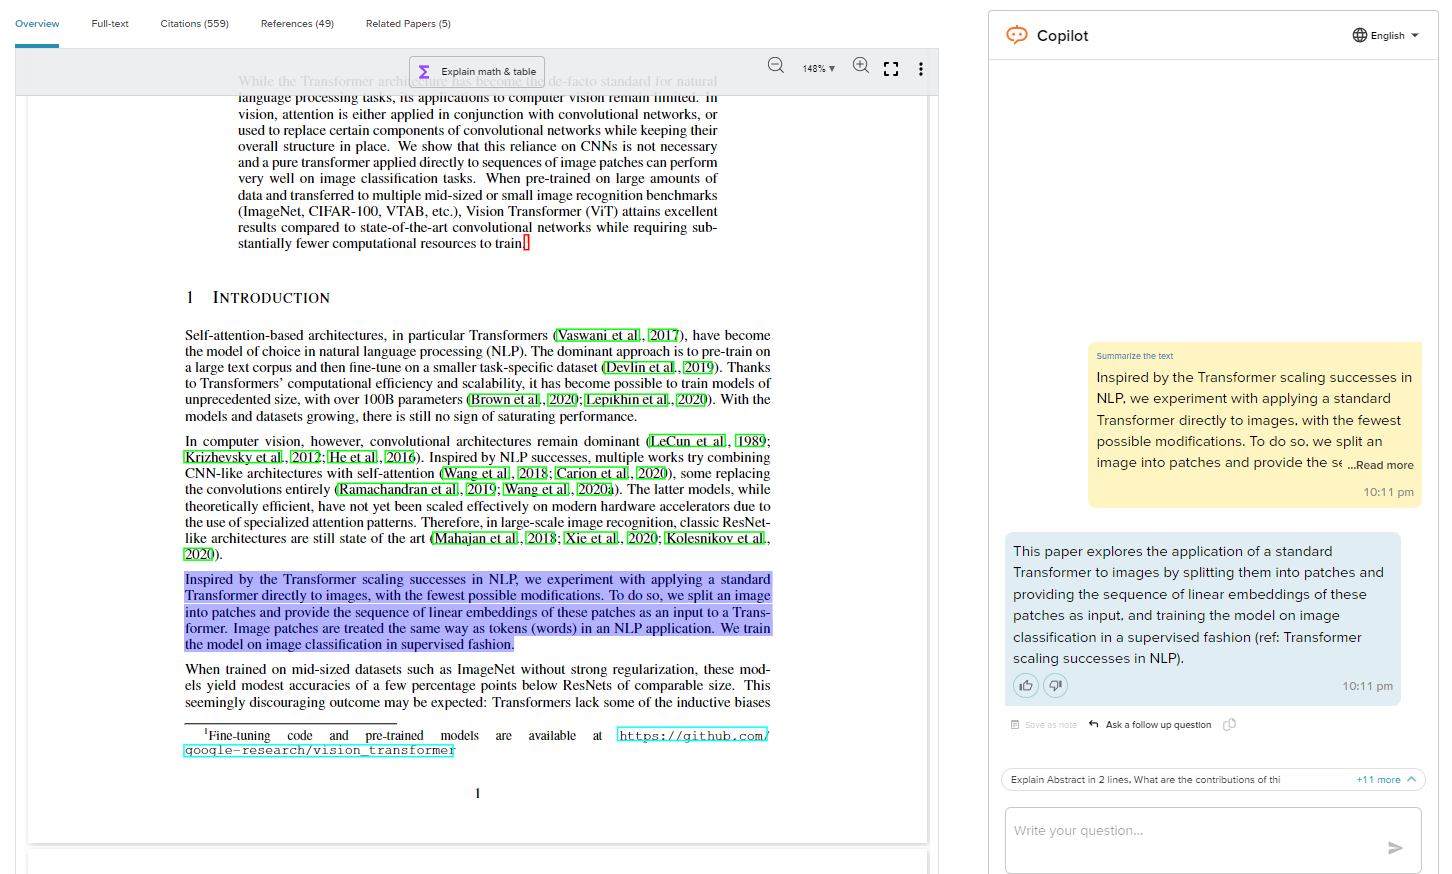
\includegraphics[width=\linewidth]{img/typeset-example.png}
	\caption{Informatie opvragen van een wetenschappelijk artikel met SciSpace}
	\label{img:scispace-example}
\end{figure}

Alle uitgeteste tools passen moeilijke woorden aan naar een eenvoudiger alternatief. O1, O3, O4 en O5 kunnen een extra definitie aan de woorden toevoegen, maar enkel wanneer er geen eenvoudiger alternatief is. Figuur \ref{img:simplish-output} toont hoe O1 een extra definitie in de voetnoot plaatst. Figuur \ref{img:scholarcy} toont aan dat O3 op taalniveau de doelgroep probeert in te schatten met \textit{rewordifying level}. O4 en O5 passen de doelgroep aan naargelang de meegegeven doelgroep in de prompt. Andere uitgeteste tools passen de woorden aan, maar bieden geen transparantie over de inschatting van de doelgroep.

\medspace

% must-have
E1, E2, E3 en O1 kunnen woorden- en synoniemenlijsten genereren. De gebruiker moet hier de moeilijke woorden handmatig selecteren. Nadien bouwt de toepassing een woordenlijst. E1 geeft de eindgebruiker de keuze waarvan E1 de definitie moet halen. O1 geeft het type woord, zoals adjectieven of werkwoord, ook mee in de woordenlijst. O4 en O5 kunnen enkel een woordenlijst genereren na een expliciete prompt. Zowel handmatige als automatische woordselectie resulteren met de geteste prompt in een woordenlijst. Andere tools zijn niet in staat om een woordenlijst te genereren. De inschatting van de doelgroep bij deze moeilijke woorden gebeurt enkel manueel.

\medspace

E1, E2 en E3 reiken de \textit{must-have} opmaakopties aan binnen de toepassing. Andere tools ontbreken personaliseerbare opmaakopties en bieden een statische webweergave aan. Ten slotte biedt geen uitgeteste tool personaliseerbare opmaakopties voor de uitvoerbestanden aan. 

\medspace

E1, E2 en E3 kunnen geen SS-technieken toepassen op de oorspronkelijke tekst. Overige uitgeteste tools kunnen zinnen inkorten door ze te splitsen. Geen van de uitgeteste tools is in staat om automatisch de tekst naar de actieve vorm te schrijven. O4 en O5 kunnen zinnen omvormen naar de actieve stem, maar enkel als de tool een extra voornaamwoord of onderwerp in de prompt meekrijgt.

\medspace

Tot slot slagen O2, O4 en O5 erin om de tekst te herschrijven als opsomming. O2 doet dit automatisch. O4 en O5 moeten deze vraag expliciet in hun prompt krijgen. De andere uitgeteste tools kunnen dit niet automatisch doen.

\subsubsection{Should-haves}

O1 en O3 tonen automatisch tekstanalyse na de vereenvoudiging van een tekst, zoals weergegeven in figuren \ref{img:simplish-output} en \ref{img:scholarcy}. Deze tools tonen het aantal zinnen, het aantal complexe woorden en het aantal lange woorden voor zowel het oorspronkelijk als het vereenvoudigde artikel. Andere tools, inclusief de verwante prompts van O4 en O5, reiken dit niet automatisch aan. 

\begin{figure}[H]
	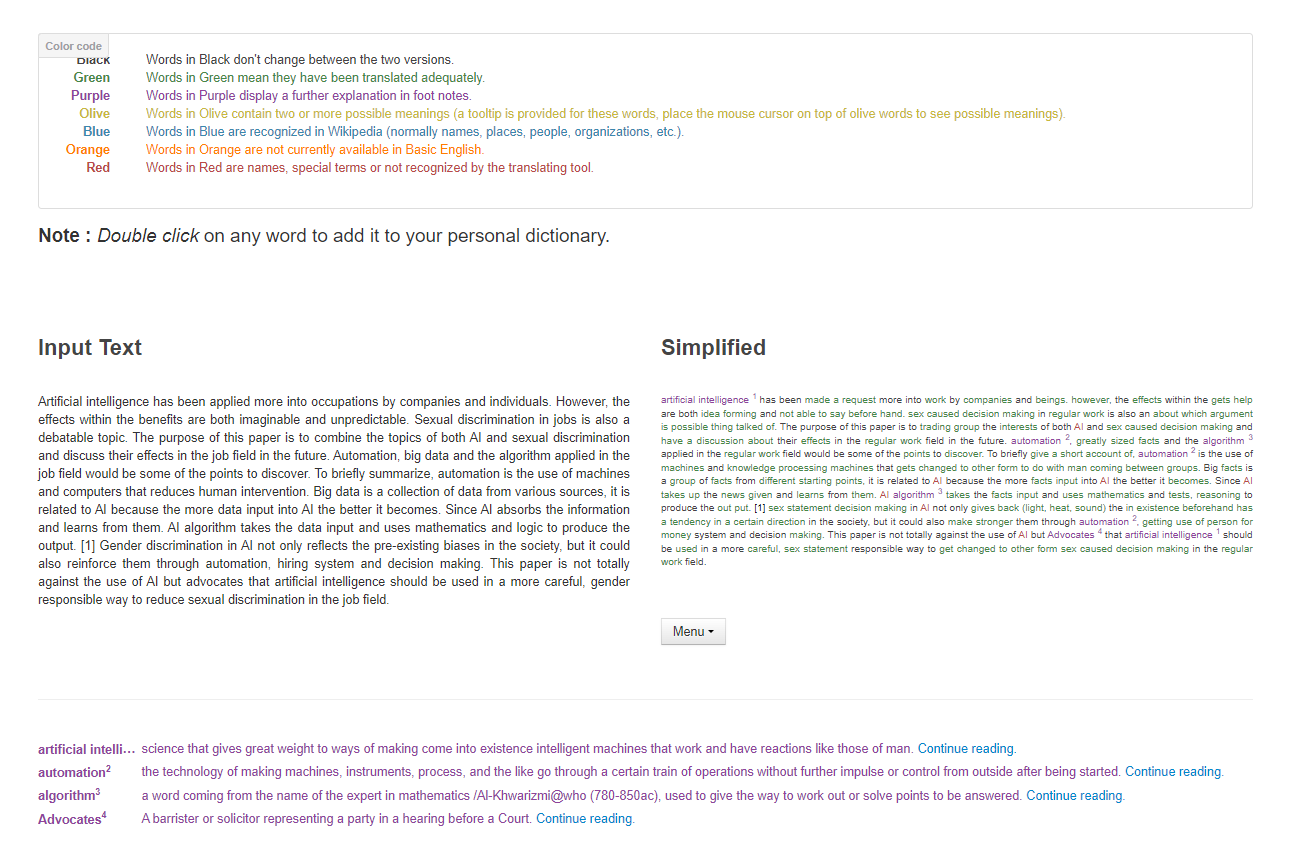
\includegraphics[width=\linewidth]{img/simplish-output.png}
	\caption{Illustratie van de tekstanalyse bij Simplish na een tekstvereenvoudiging.}
	\label{img:simplish-output}
\end{figure}

\begin{figure}[H]
	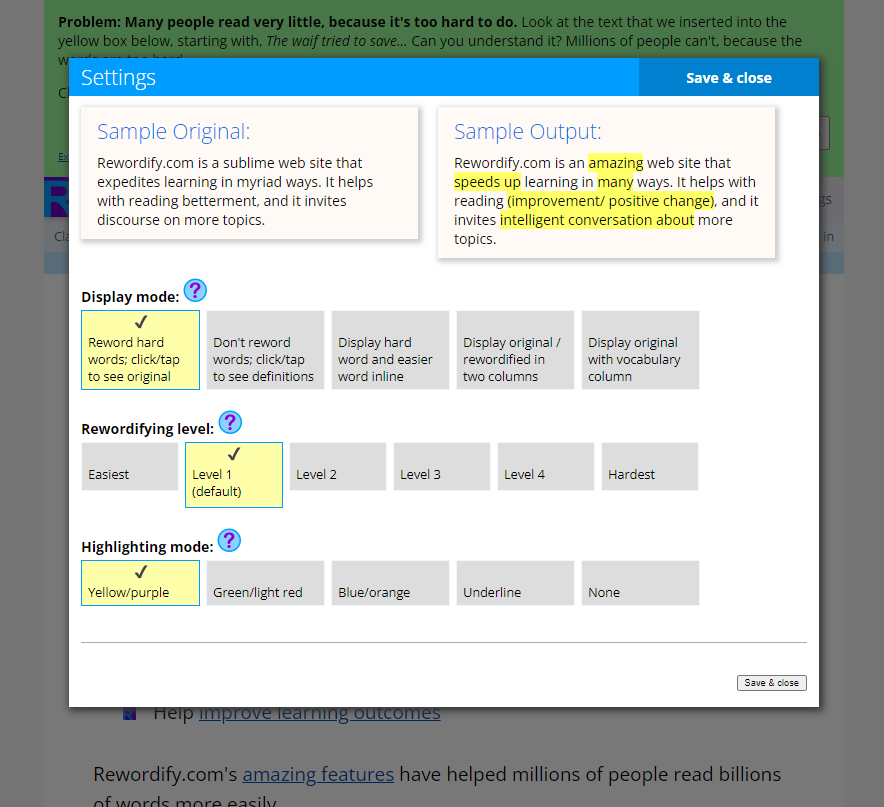
\includegraphics[width=\linewidth]{img/scholarcy-attempt.png}
	\caption{Illustratie van de tekstanalyse bij Rewordify.}
	\label{img:scholarcy}
\end{figure}

Alle uitgeteste tools, met uitzondering op O1, O4 en O5, bieden een manier aan om zonder tussenstap pdf-bestanden op te slaan. Geen toepassing biedt een functionaliteit aan om de vereenvoudigde versie als docx-bestand op te slaan.

\medspace

De requirementsanalyse kan niet achterhalen of de toepassingen gebruik maken van OCR. Wel maakt O2 gebruik van een andere inlees-techniek dan de andere tools. Zo kan het systeem alle uitgeteste wetenschappelijke artikelen inlezen. De gebruiker markeert enkel aanpassingen in het artikel, terwijl de uitvoer rechts in beeld komt. Zo kan de gebruiker de aanpassing niet zien. Daarentegen beschikken O1 en O3 over een weergave waarbij de eindgebruiker duidelijk de verschillen tussen oorspronkelijk en vereenvoudigd kan zien. Andere uitgeteste tools maken geen gebruik van deze weergave.

\subsubsection{Could-haves}

De geteste tools beschikken over de nodige functionaliteiten om gebruikerfeedback te geven. Zo voeren de uitgeteste tools pop-ups toe om de eindgebruiker attent te maken van een aanpassing. O4 en O5 bieden dit echter niet aan. Vervolgens zijn O4 en O5 de enige geteste tools die tekst in een tabelformaat kunnen schrijven, maar enkel na een expliciete prompt. Daarnaast beschikt geen van de geteste tools over een functionaliteit om automatisch de moeilijke woorden of vakterminologie op te halen uit een tekst. O4 en O5 gaven de woordenlijst in tabelvorm terug. Daarnaast kunnen O4 en O5 dit enkel met een expliciete prompt. O1, O2, O3, O4 en O5 kunnen extraherende en abstraherende samenvattingen maken van de oorspronkelijke tekst. E1, E2 en E3 kunnen een extraherende samenvatting van de tekst maken, maar enkel na een handmatige selectie van de zinnen. Enkel O4 en O5 kunnen een gekregen tekst herschrijven. Tot slot kunnen O1, O2, O4 en O5 onregelmatige werkwoorden wegwerken. Andere toepassingen kunnen dit niet uitvoeren.


\subsubsection{Wont-haves}

O4, O5 beschikken over een mobiele versie. O1, O2 en O3 kunnen gebruikers via een mobiel apparaat bekijken, maar leent geen speciale interface voor deze gebruikers toe. E1, E2 en E3 bieden geen mobiele versie aan. Enkel E1, E2 en E3 beschikken over luistersoftware. Browser bevatten een ingebouwde luistertool, maar geen van de geteste tools beschikt over \textit{text-to-speech} systeem. Tot slot beschikken de geteste toepassingen over geen integratie met andere spelcheckers. De browserextensie van Grammarly werkt bij zowel O1, O2, O3, O4 en O5.


\section{Geschikte taalmodel voor gepersonaliseerde tekstvereenvoudiging met ATS}

De vergelijkende studie evalueert de uitvoer van de uitgeteste taallmodellen, opgesomd in \ref{table:vergelijkende-studie-taalmodellen}, met een machinale en een menselijke beoordeling. Zo achterhaalt deze onderzoeksmethode welk taalmodel of LLM beter aansluit bij het aanbieden van gepersonaliseerde ATS voor scholieren met dyslexie in de derde graad van het middelbaar onderwijs. 

\subsubsection{Machinale beoordeling van de vereenvoudigde teksten}

\medspace

Tabel \ref{table:resultaten-aantal-zinnen} geeft het aantal zinnen per (vereenvoudigd) artikel. De MTS-referentieteksten bevatten minder zinnen dan het oorspronkelijk artikel. Het aantal zinnen na ATS met T1, T2 en T3 is gehalveerd tot minder dan een kwart van oorspronkelijke hoeveelheid zinnen. Enkel T4P2 genereert meer zinnen dan de oorspronkelijke versie van A1 na ATS. T4P2 genereert bij zowel A1 als A2 meer zinnen vergeleken met de andere geteste taalmodellen. T2 daarentegen genereert bij beide artikelen het minst aantal zinnen.

\medspace

% Daarnaast gebruiken T1, T2 en T3 gemiddeld minder woorden per zin dan het oorspronkelijke artikel. Alleen P3 van T4 slaagt erin om gemiddeld minder woorden per zin te gebruiken dan de oorspronkelijke en de referentieteksten van zowel leerlingen en de referentieteksten van leerkrachten, vergeleken met P1 en P2 die elk gemiddeld meer dan 19 woorden per zin gebruiken, zoals te zien is in figuren . 

\begin{table}[h]
	\centering
	\begin{tabular}{ | m{3cm} | m{3cm} | m{3cm} | } 
		\hline
		\textbf{Bron} & \textbf{#Zinnen in A1} & \textbf{#Zinnen in A2} \\
		\hline
		Oorspronkelijk & 78  & 159 \\ 
		\hline
		MTS (door leerkracht) & 43 & 45 \\
		\hline
		MTS (door leerling) & n.v.t. & 50 \\
		\hline
		T1 & 26 & 24 \\
		\hline
		T2 & 11 & 7 \\
		\hline
		T3 & 67 & 130 \\
		\hline
		T4 P1 & 61 & 98 \\
		\hline
		T4 P2 & 89 & 133 \\
		\hline
		T4 P3 & 39 & 55 \\
		\hline
	\end{tabular}
	\caption{Aantal zinnen (gemeten met Spacy sentence embeddings) per tekst.}
	\label{table:resultaten-aantal-zinnen}
\end{table}

\begin{figure}[H]
	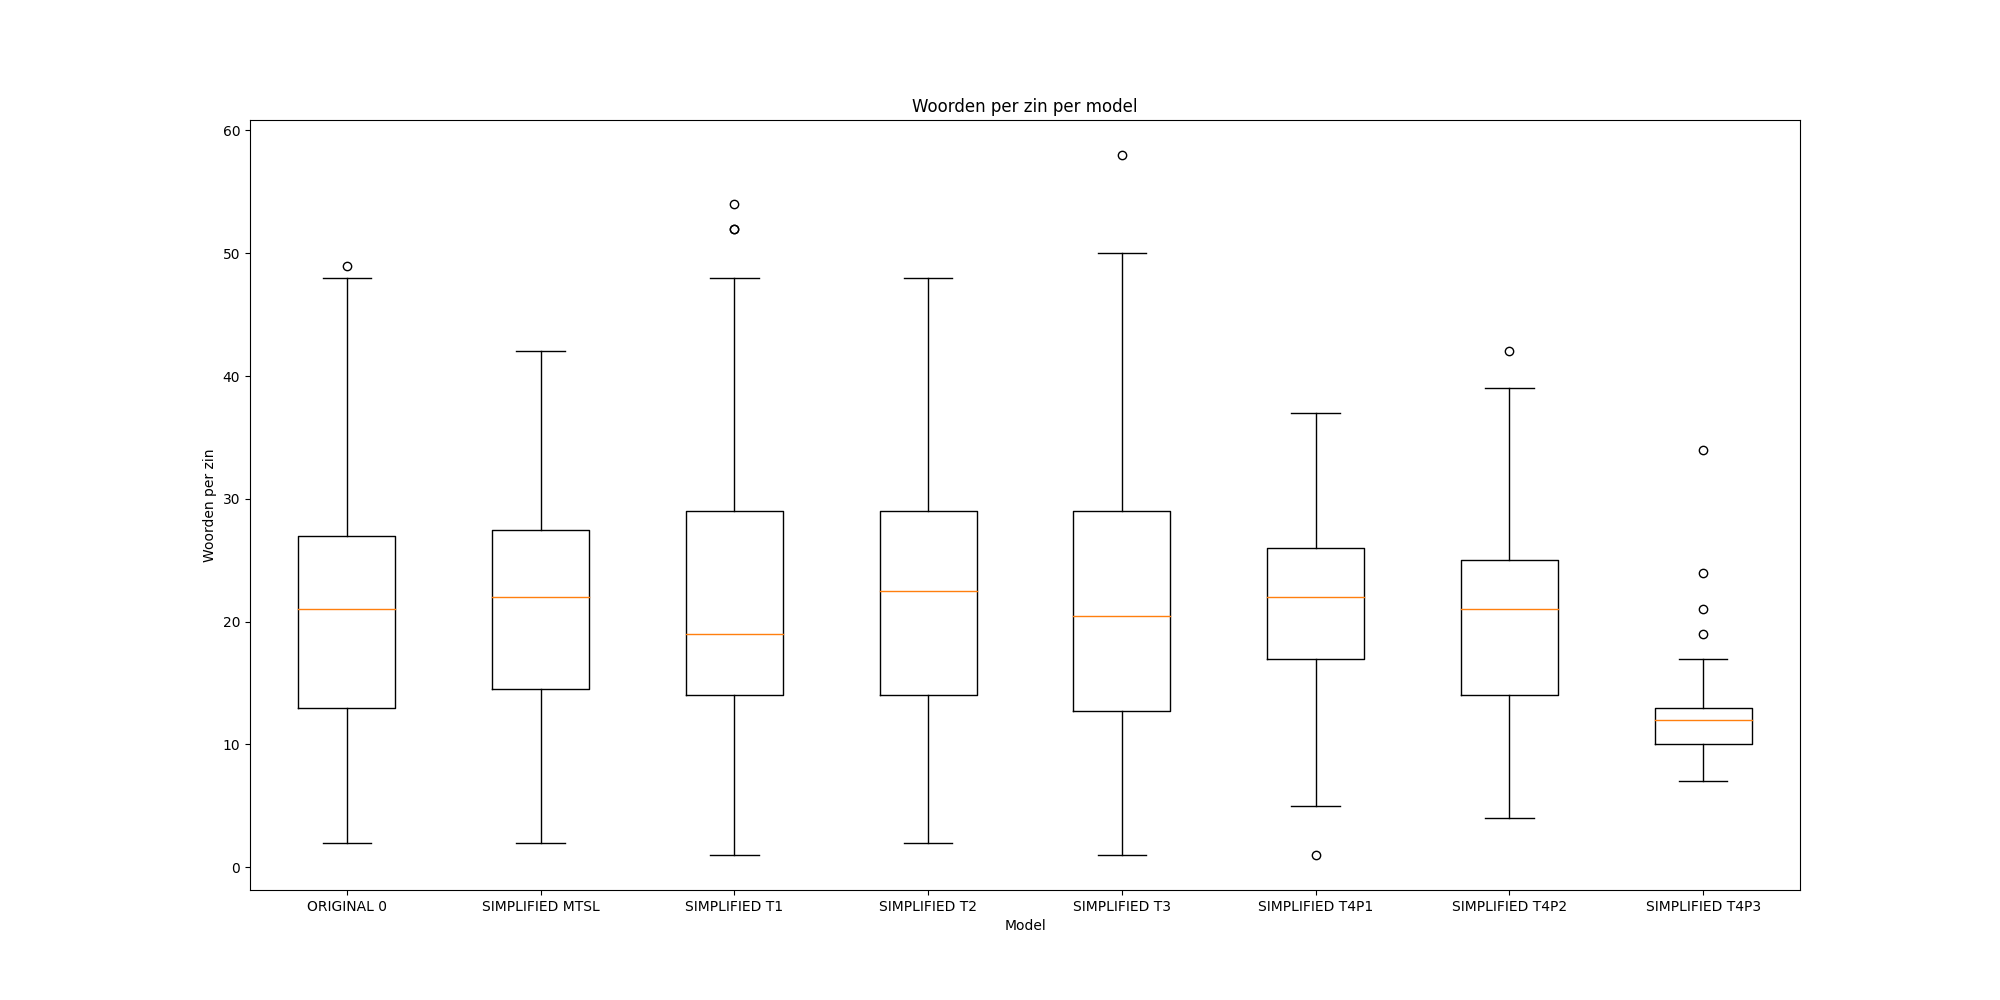
\includegraphics[width=\linewidth]{img/boxplot-avg-a1.png}
	\caption{Overzicht van het minimum, maximum en gemiddeld aantal woorden per zin per model in A1.}
	\label{img:boxplot-min-max-avg-words-a1}
\end{figure}

\begin{figure}[H]
	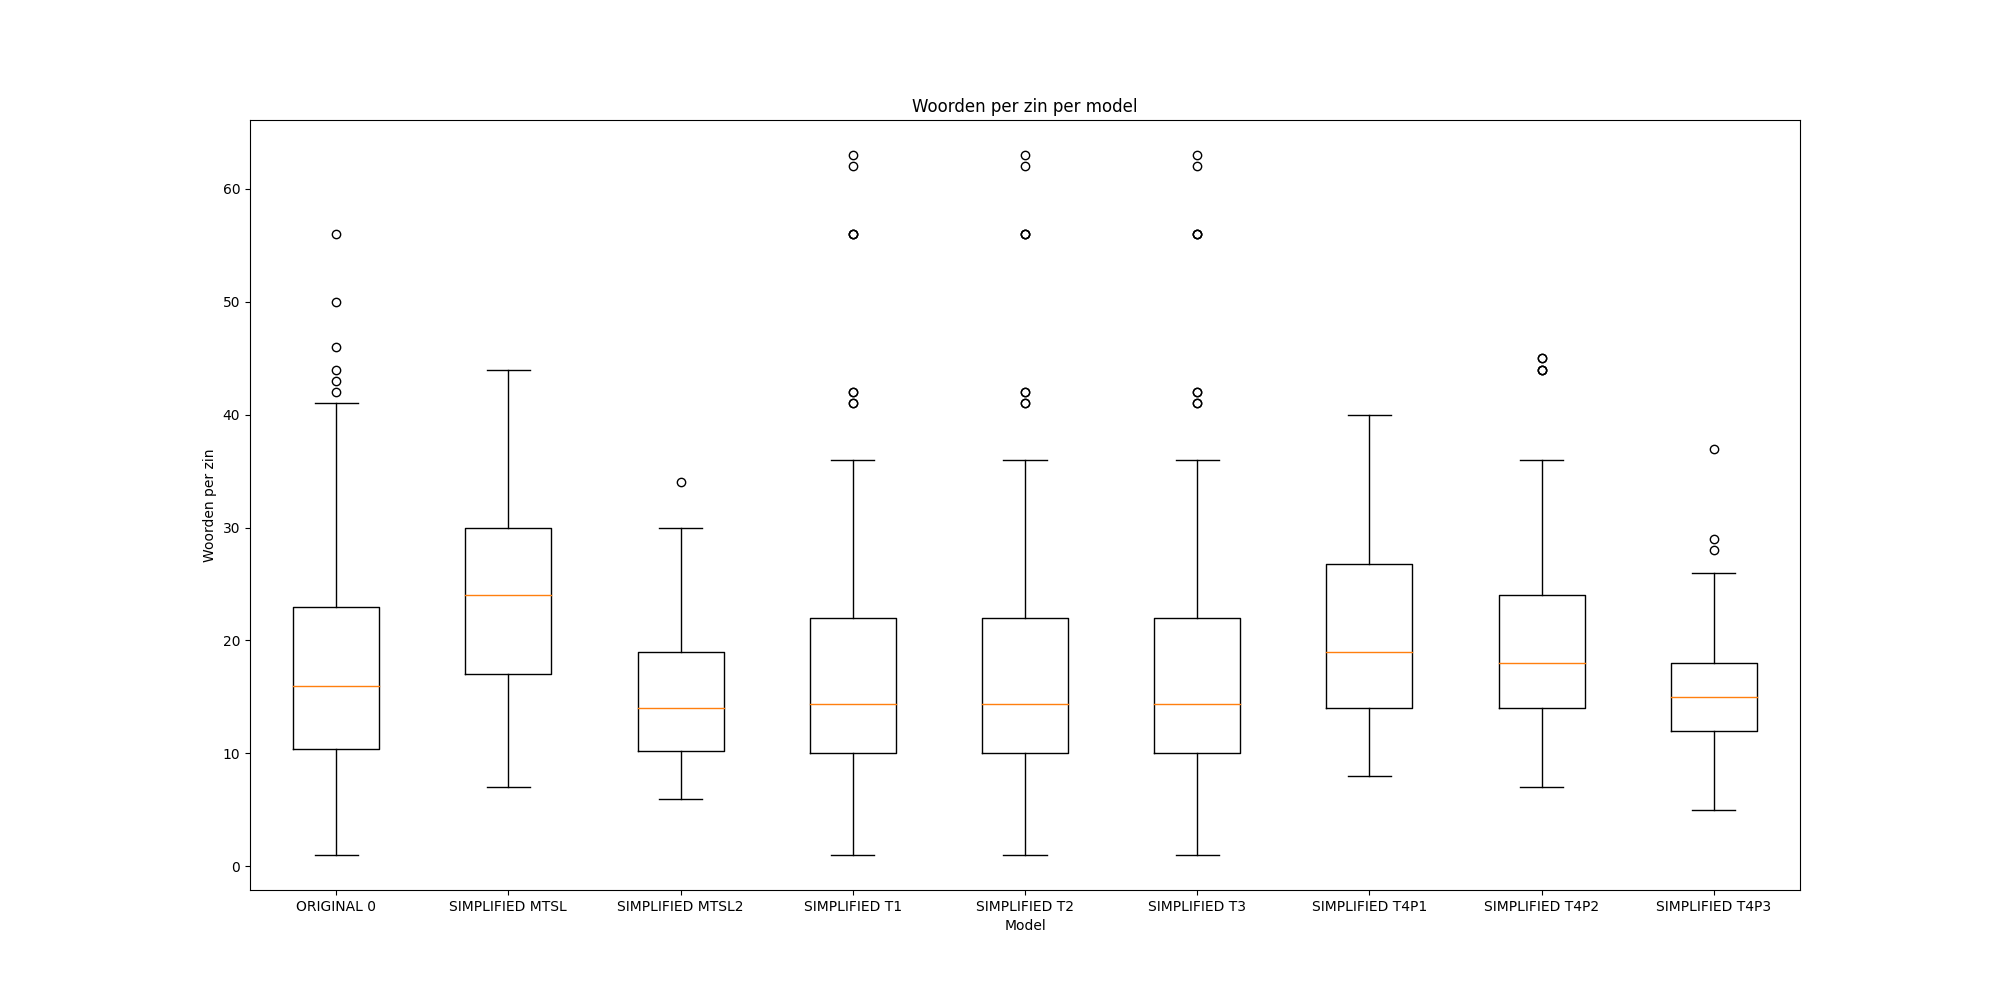
\includegraphics[width=\linewidth]{img/boxplot-avg-a2.png}
	\caption{Overzicht van het minimum, maximum en gemiddeld aantal woorden per zin per model in A2.}
	\label{img:boxplot-min-max-avg-words-a2}
\end{figure}

De FRE-scores van alle geteste taalmodellen en MTS-referentieteksten zijn niet significant hoger of lager dan die van OG, zoals weergegeven in figuren \ref{img:boxplot-fre-a1} en \ref{img:boxplot-fre-a2}. Gemiddeld bevinden alle versies van het wetenschappelijk artikel zich tussen 20 en 50. Zonder \textit{outliers} beperkt T3 de FRE van alle zinnen tot hoogstens 40. T3, T4P1, T4P2 en T4P3 genereren zinnen met een hogere FRE dan OG en MTSL. 

\begin{figure}[H]
	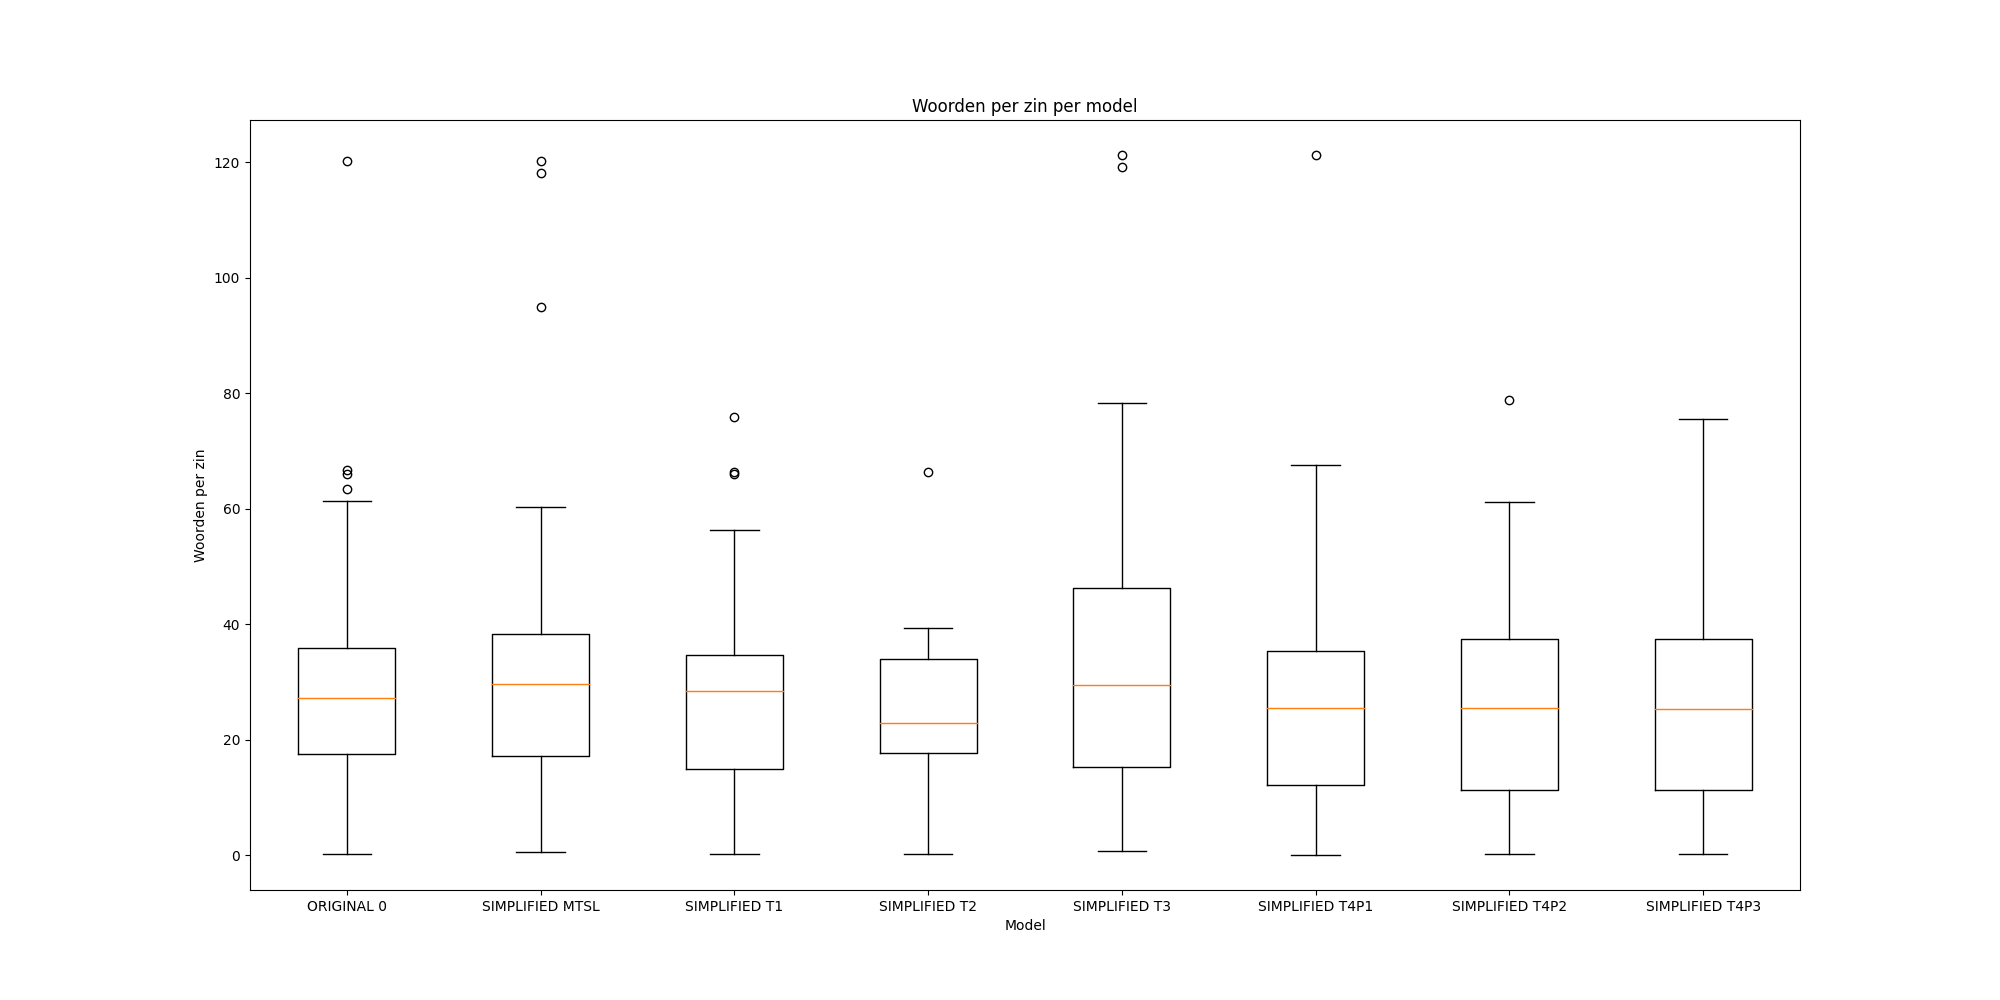
\includegraphics[width=\linewidth]{img/boxplot-fre-a1.png}
	\caption{Boxplot van de FRE-scores voor A1.}
	\label{img:boxplot-fre-a1}
\end{figure}

\begin{figure}[H]
	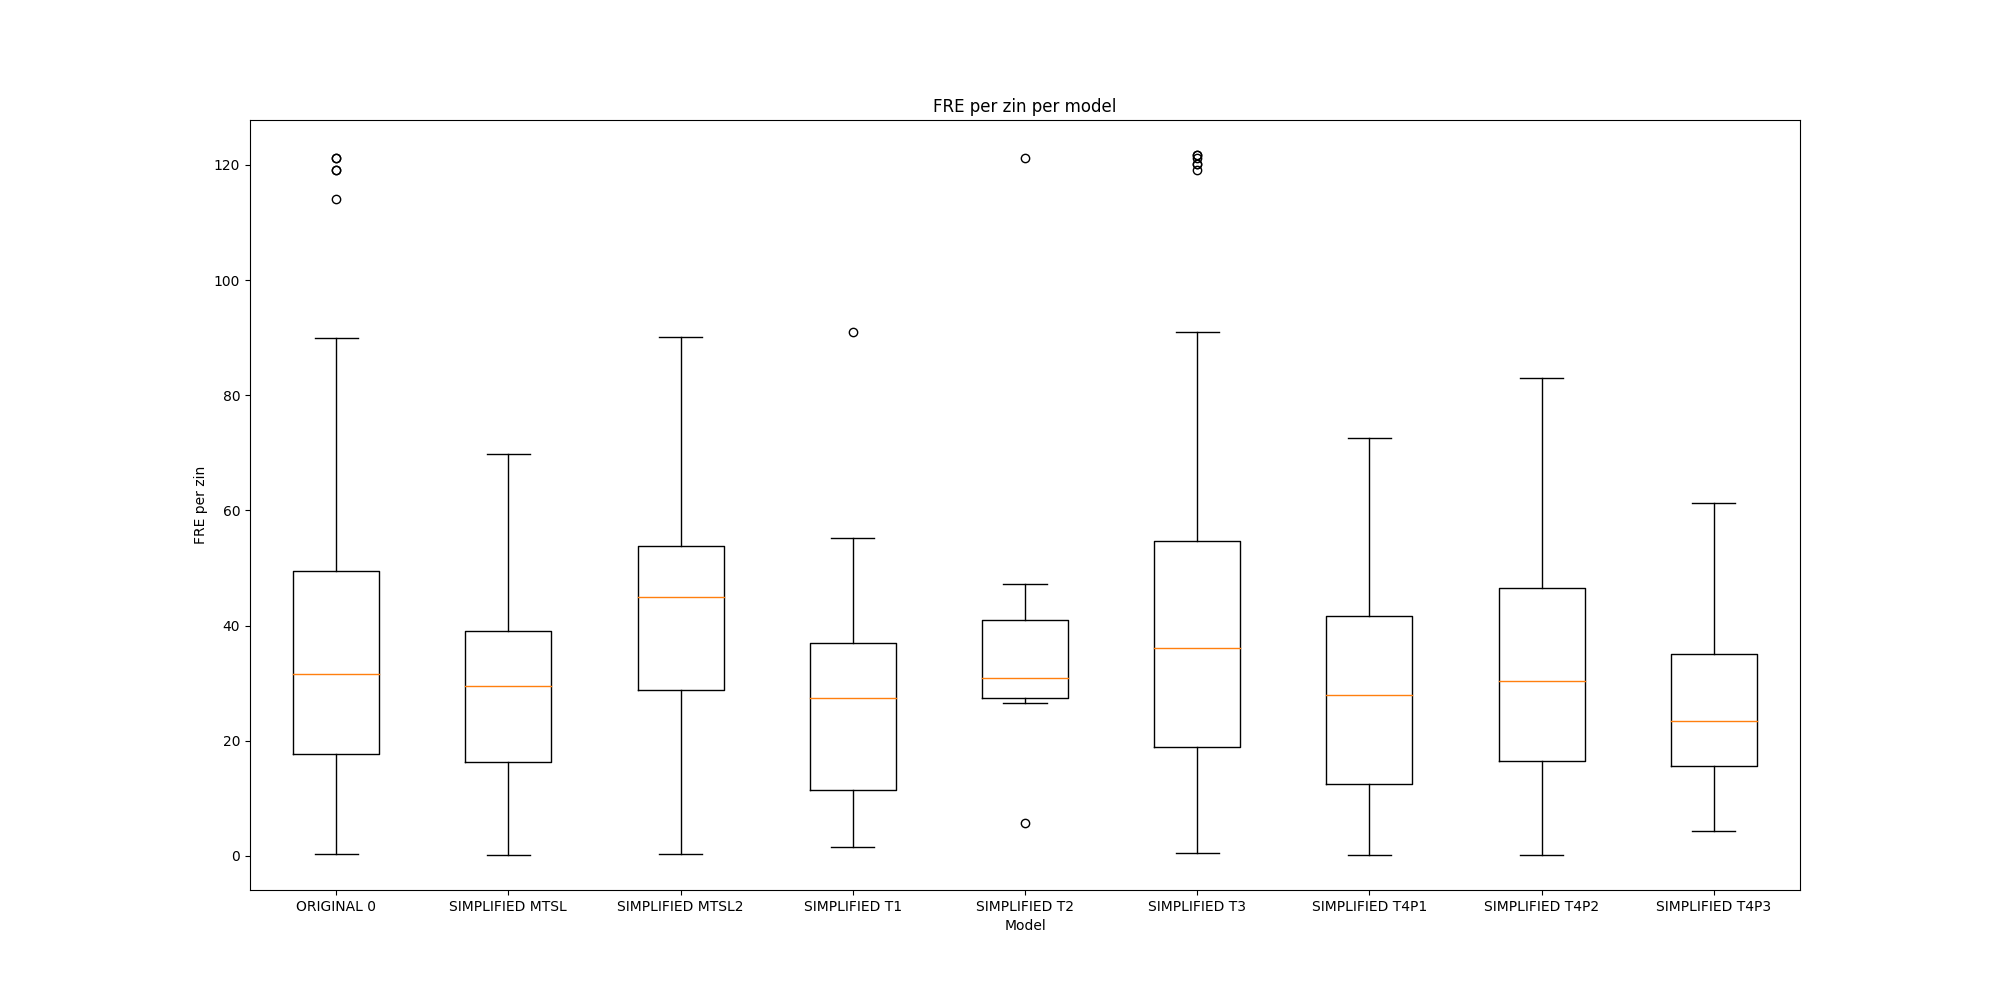
\includegraphics[width=\linewidth]{img/boxplot-fre-a2.png}
	\caption{Boxplot van de FRE-scores voor A2.}
	\label{img:boxplot-fre-a2}
\end{figure}

De FOG-scores van alle geteste taalmodellen en MTS-referentieteksten zijn niet significant hoger of lager bij de vereenvoudigde wetenschappelijke artikelen, zoals gevisualiseerd in figuren \ref{img:boxplot-fog-a1} en \ref{img:boxplot-fog-a2}. De zinnen van MTSL2 en T2 scoren een gemiddeld lagere FOG-score dan OG. T2 scoort het laagste gemiddelde van alle taalmodellen. Het gemiddelde van T2 ligt tussen 10 en 12. Tot slot scoren MTSL en andere taalmodellen gemiddeld hoger dan OG. Tot slot genereren de taalmodellen geen zinnen met een hogere FOG-score dan OG.

\begin{figure}[H]
	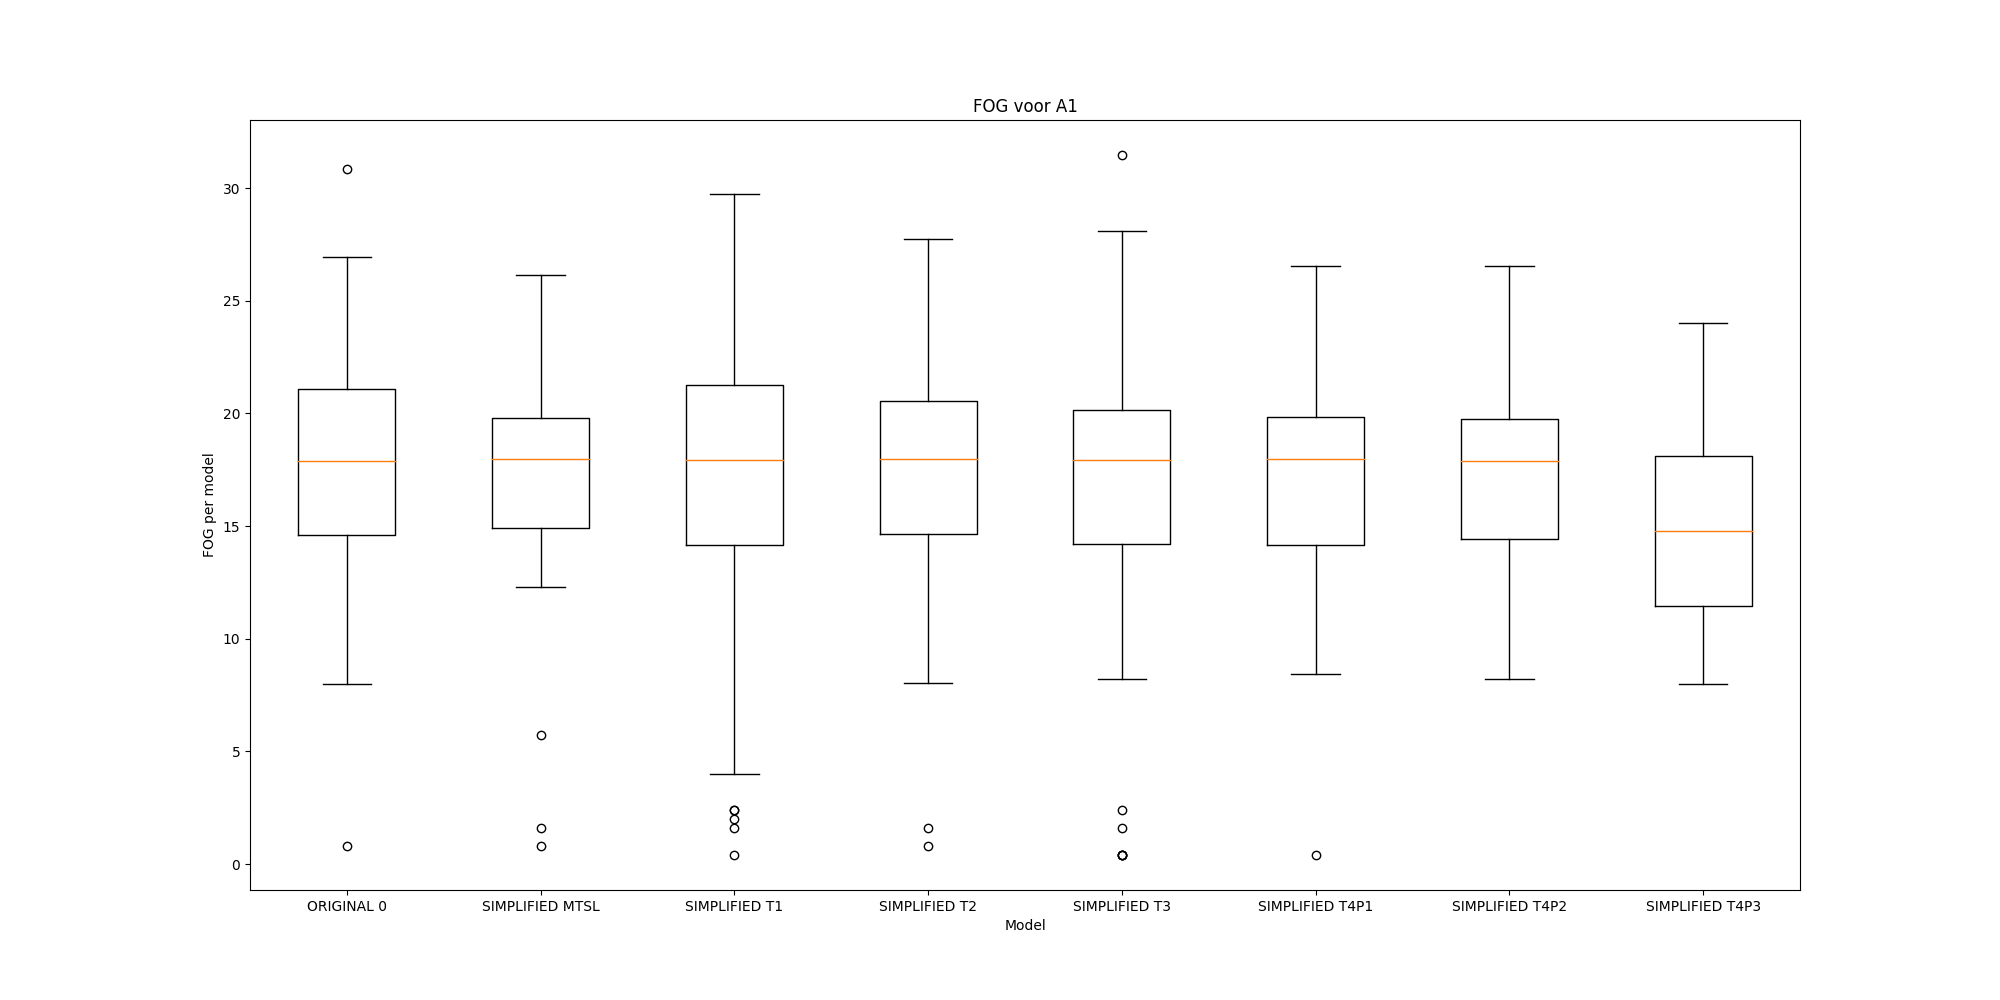
\includegraphics[width=\linewidth]{img/boxplot-fog-a1.png}
	\caption{Boxplot van de FOG-scores voor A1.}
	\label{img:boxplot-fog-a1}
\end{figure}

\begin{figure}[H]
	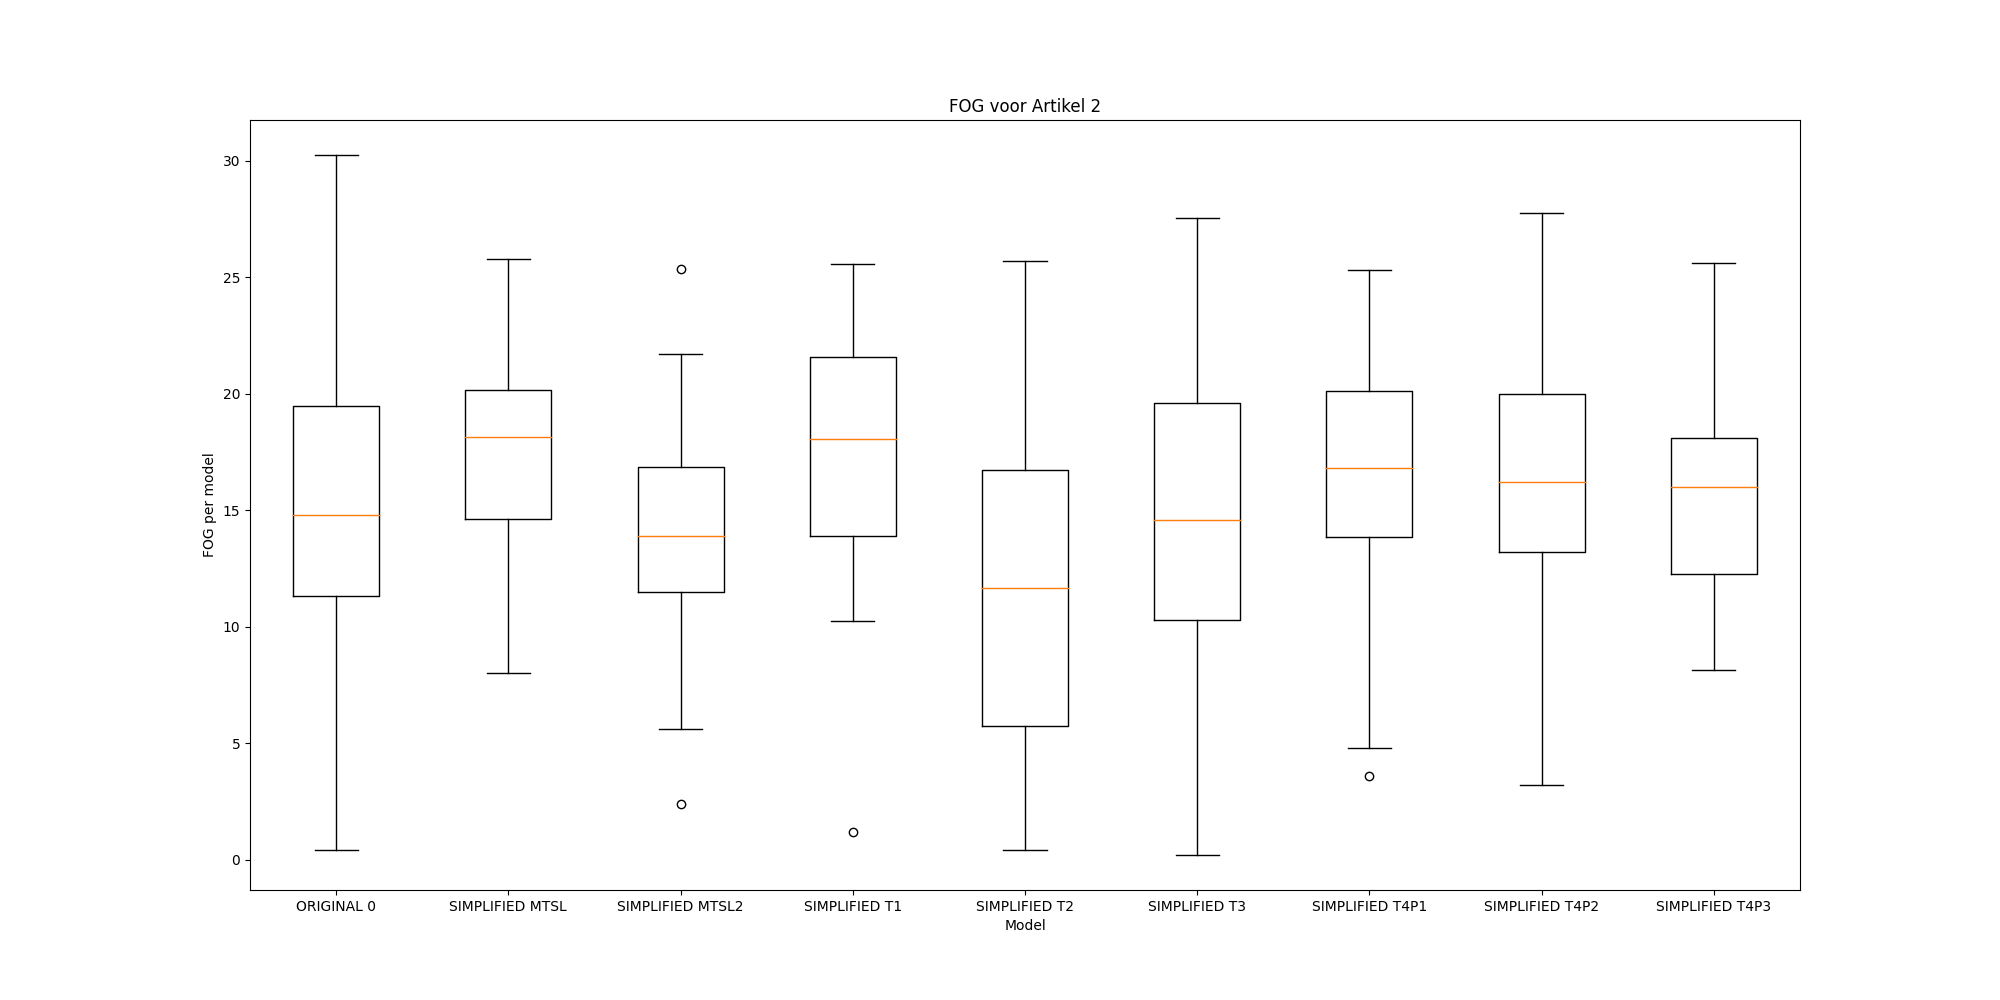
\includegraphics[width=\linewidth]{img/boxplot-fog-a2.png}
	\caption{Boxplot van de FOG-scores voor A2.}
	\label{img:boxplot-fog-a2}
\end{figure}

Figuren \ref{img:violinplot-long-a1} en \ref{img:violinplot-long-a2} tonen het aantal gegenereerde complexe woorden (volgens DCI) per zin aan. Daarnaast genereren T1, T2 en T3 meer complexe woorden vergeleken met T4, MTSL en OG. Figuren \ref{img:violinplot-complex-a1} en \ref{img:violinplot-complex-a2} illustreren deze verschillen. Bij A1 genereert T4P3 significant minder complexe woorden per zin dan de andere taalmodellen. Bij A2 is er geen significant verschil tussen de taalmodellen.

\begin{figure}[H]
	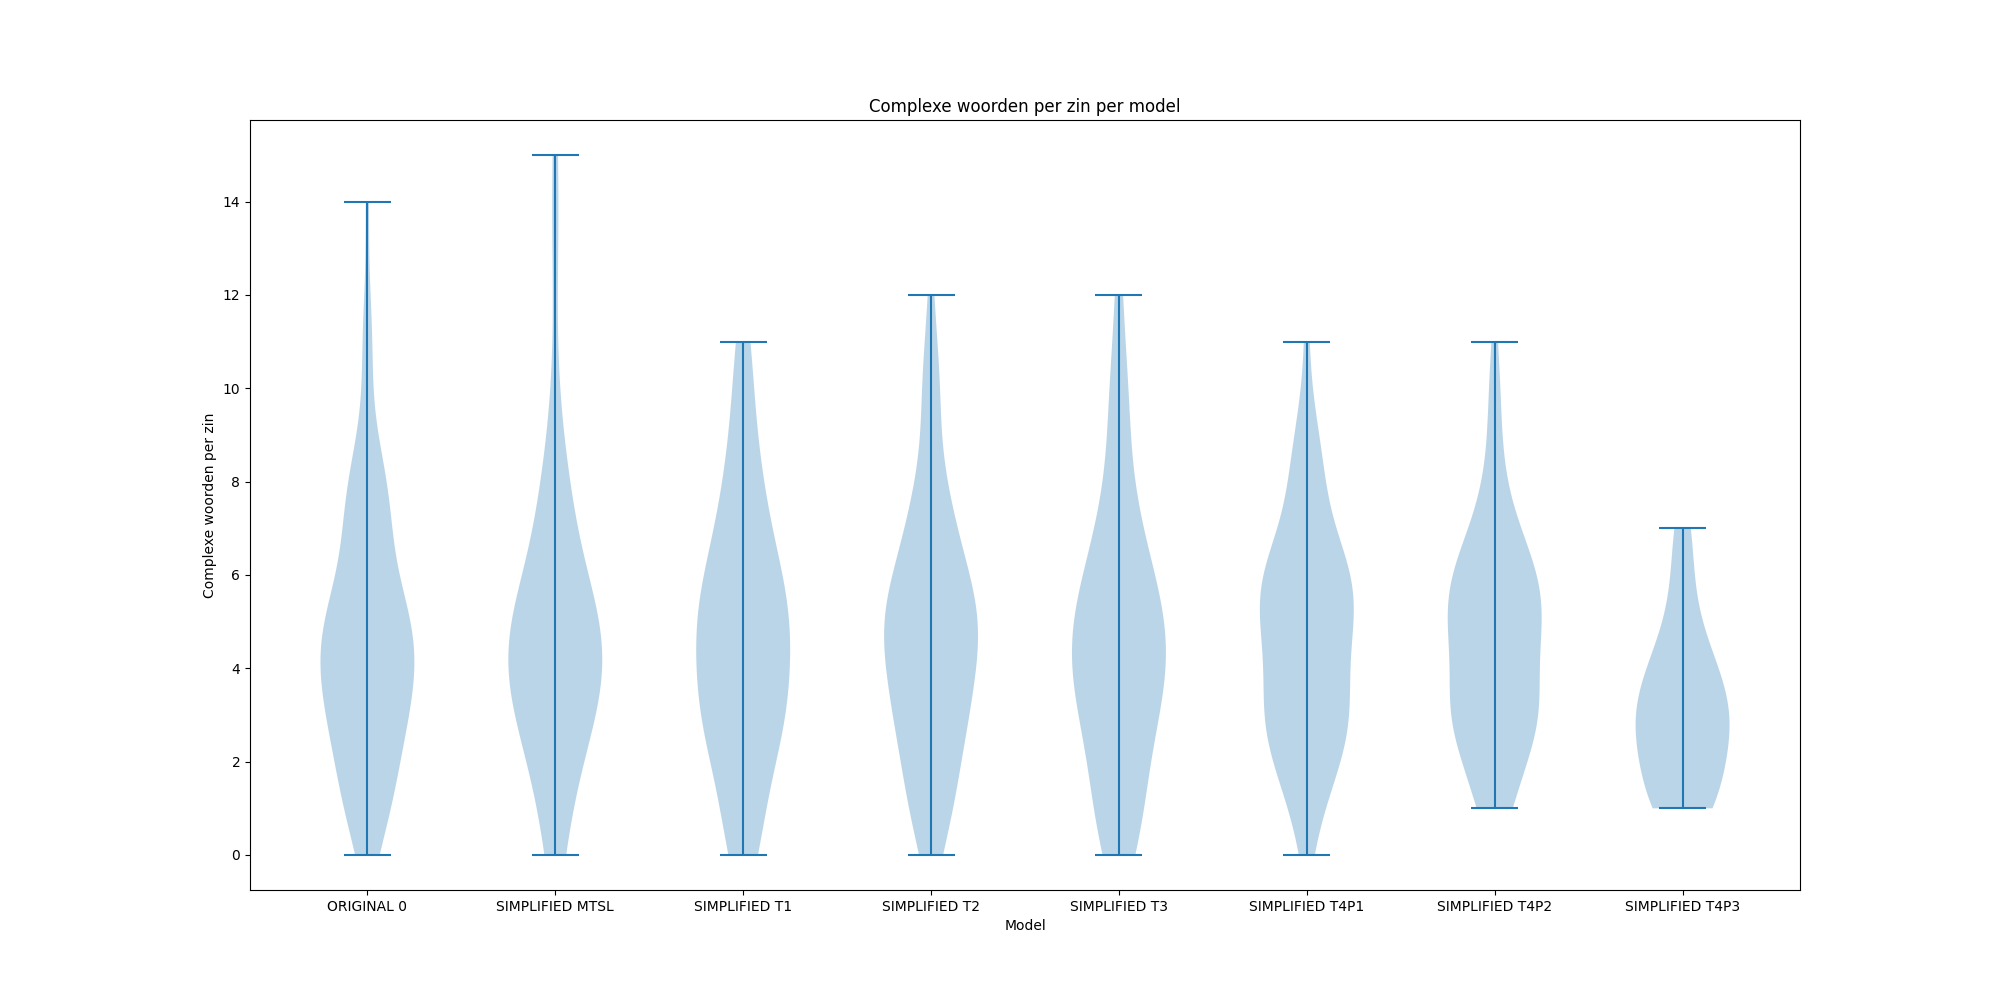
\includegraphics[width=\linewidth]{img/violinplot-complex-a1.png}
	\caption{Een violinplot van het aantal complexe woorden per zin, gegroepeerd op model voor A1.}
	\label{img:violinplot-complex-a1}
\end{figure}

\begin{figure}[H]
	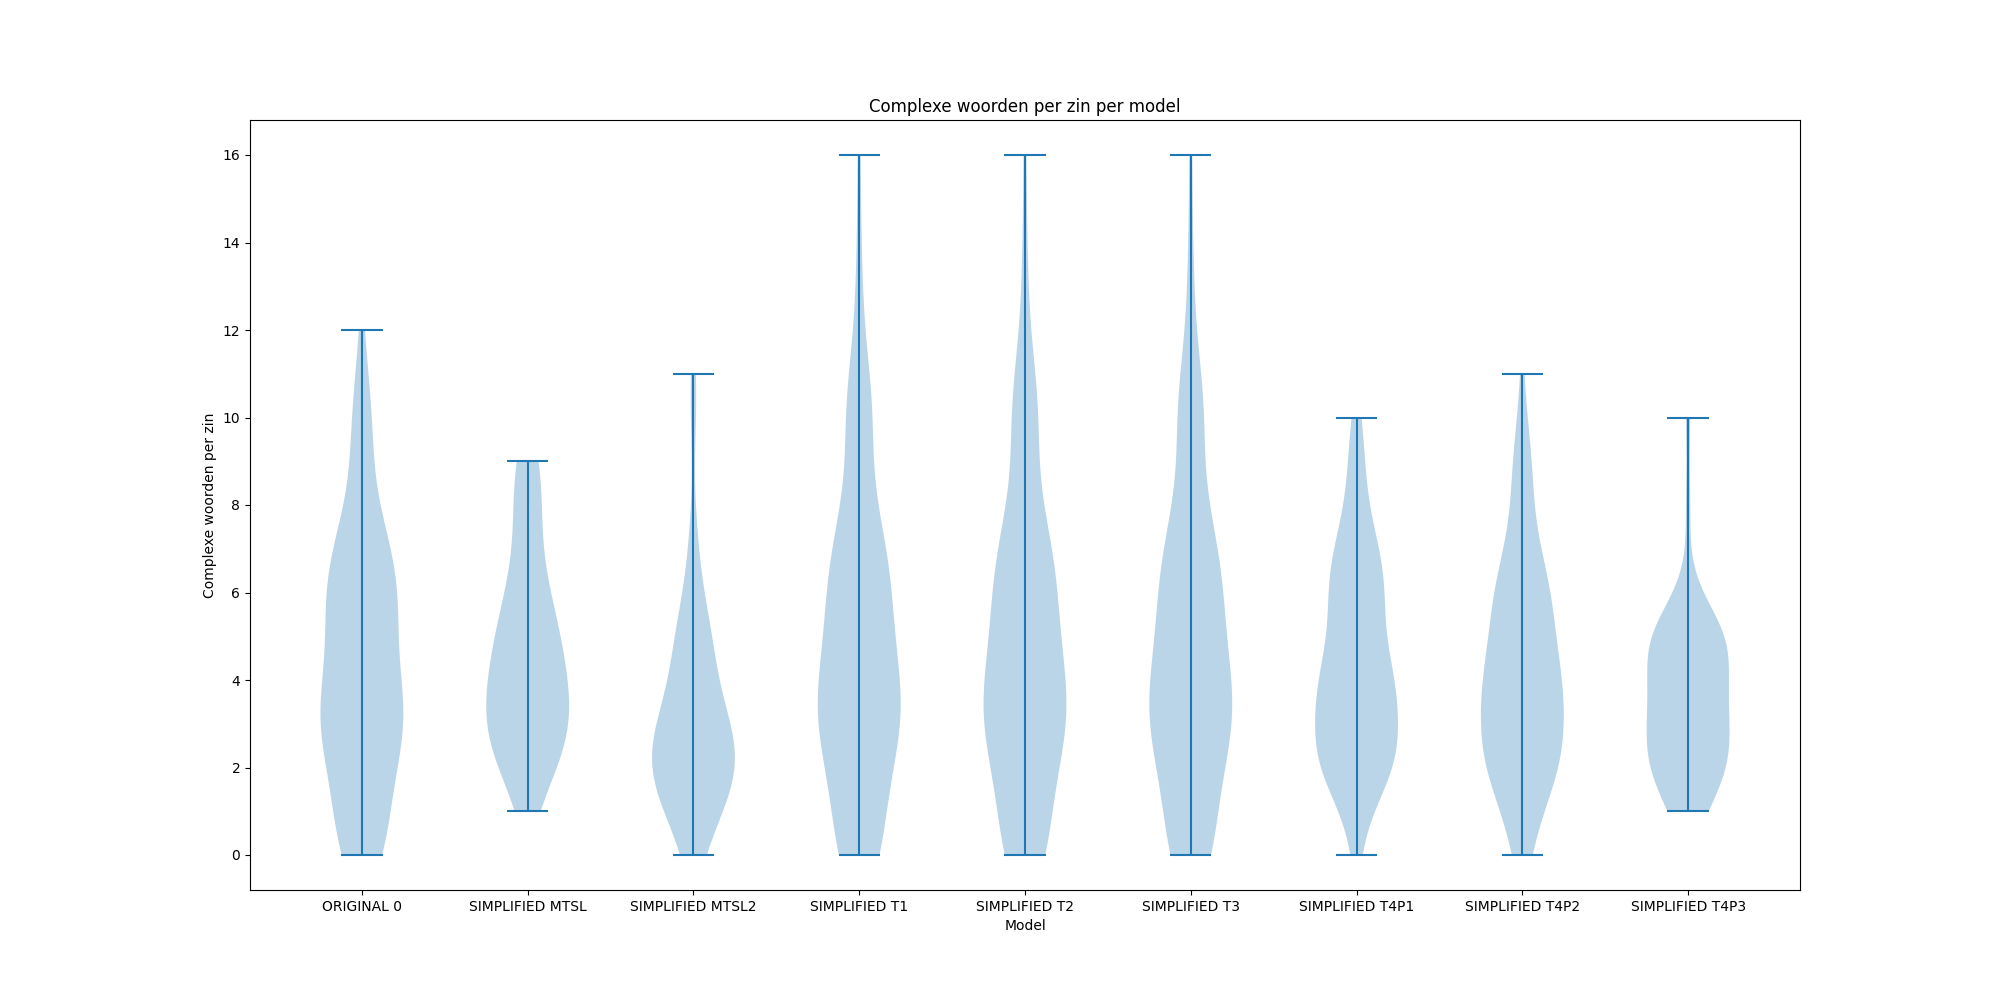
\includegraphics[width=\linewidth]{img/violinplot-complex-a2.png}
	\caption{Een violinplot van het aantal complexe woorden per zin, gegroepeerd op model voor A2.}
	\label{img:violinplot-complex-a2}
\end{figure}

Vervolgens visualiseren figuren \ref{img:violinplot-long-a1} en \ref{img:violinplot-long-a2} het aantal lange woorden (ofwel een woord met meer dan vier lettergrepen) per zin. MTSL, T2, T4P1, T4P2 en T4P3 genereren niet meer lange woorden per zin dan OG bij A1.

\begin{figure}[H]
	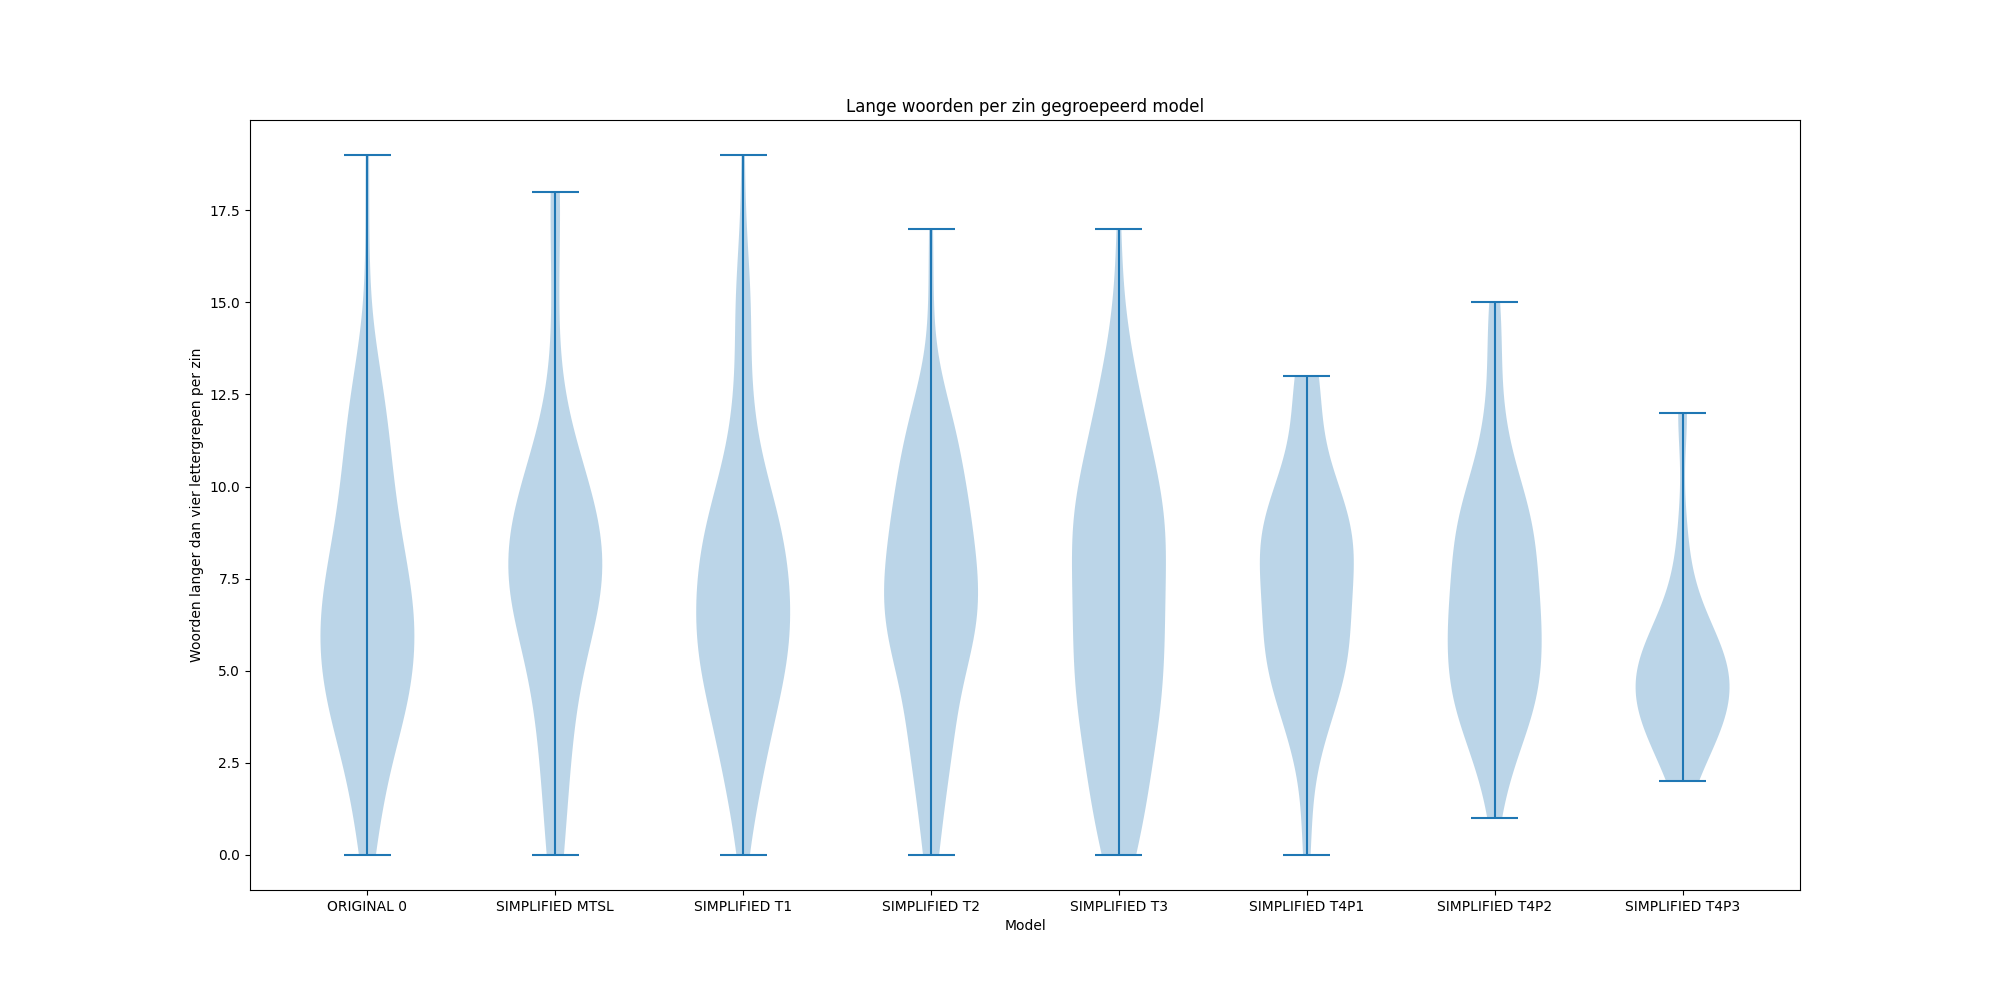
\includegraphics[width=\linewidth]{img/violinplot-long-a1.png}
	\caption{Een violinplot van het aantal lange woorden per zin, gegroepeerd op model voor A1.}
	\label{img:violinplot-long-a1}
\end{figure}

\begin{figure}[H]
	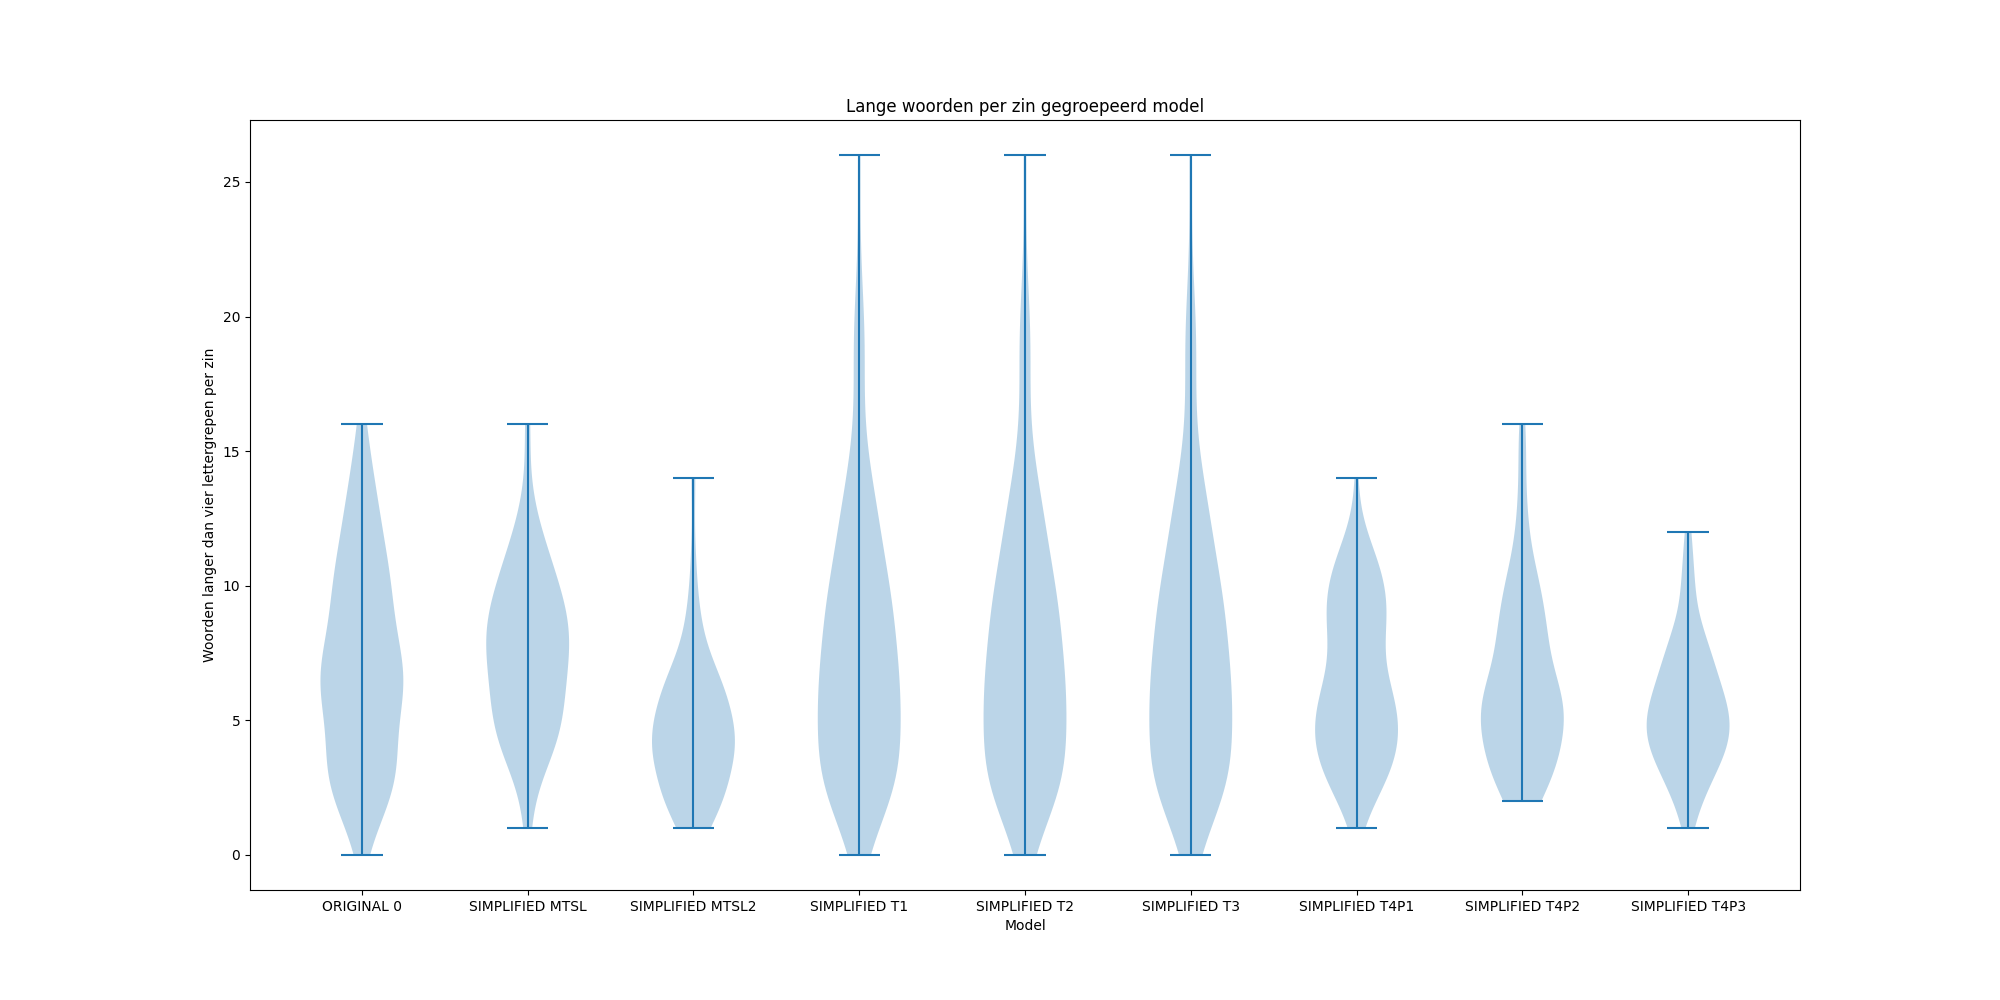
\includegraphics[width=\linewidth]{img/violinplot-long-a2.png}
	\caption{Een violinplot van het aantal lange woorden per zin, gegroepeerd op model voor A2.}
	\label{img:violinplot-long-a2}
\end{figure}

Vervolgens tonen figuren \ref{img:histplot-aux-a1} en \ref{img:histplot-aux-a2} het aantal hulpwerkwoorden in de tekst. Deze figuren zijn geen absolute percentages en houden geen rekening met het aantal zinnen. Ten slotte tonen \ref{img:histplot-aux-a1} en \ref{img:histplot-aux-a2} het aantal vervoegingen van het werkwoord 'zijn' aan. 

\begin{figure}[H]
	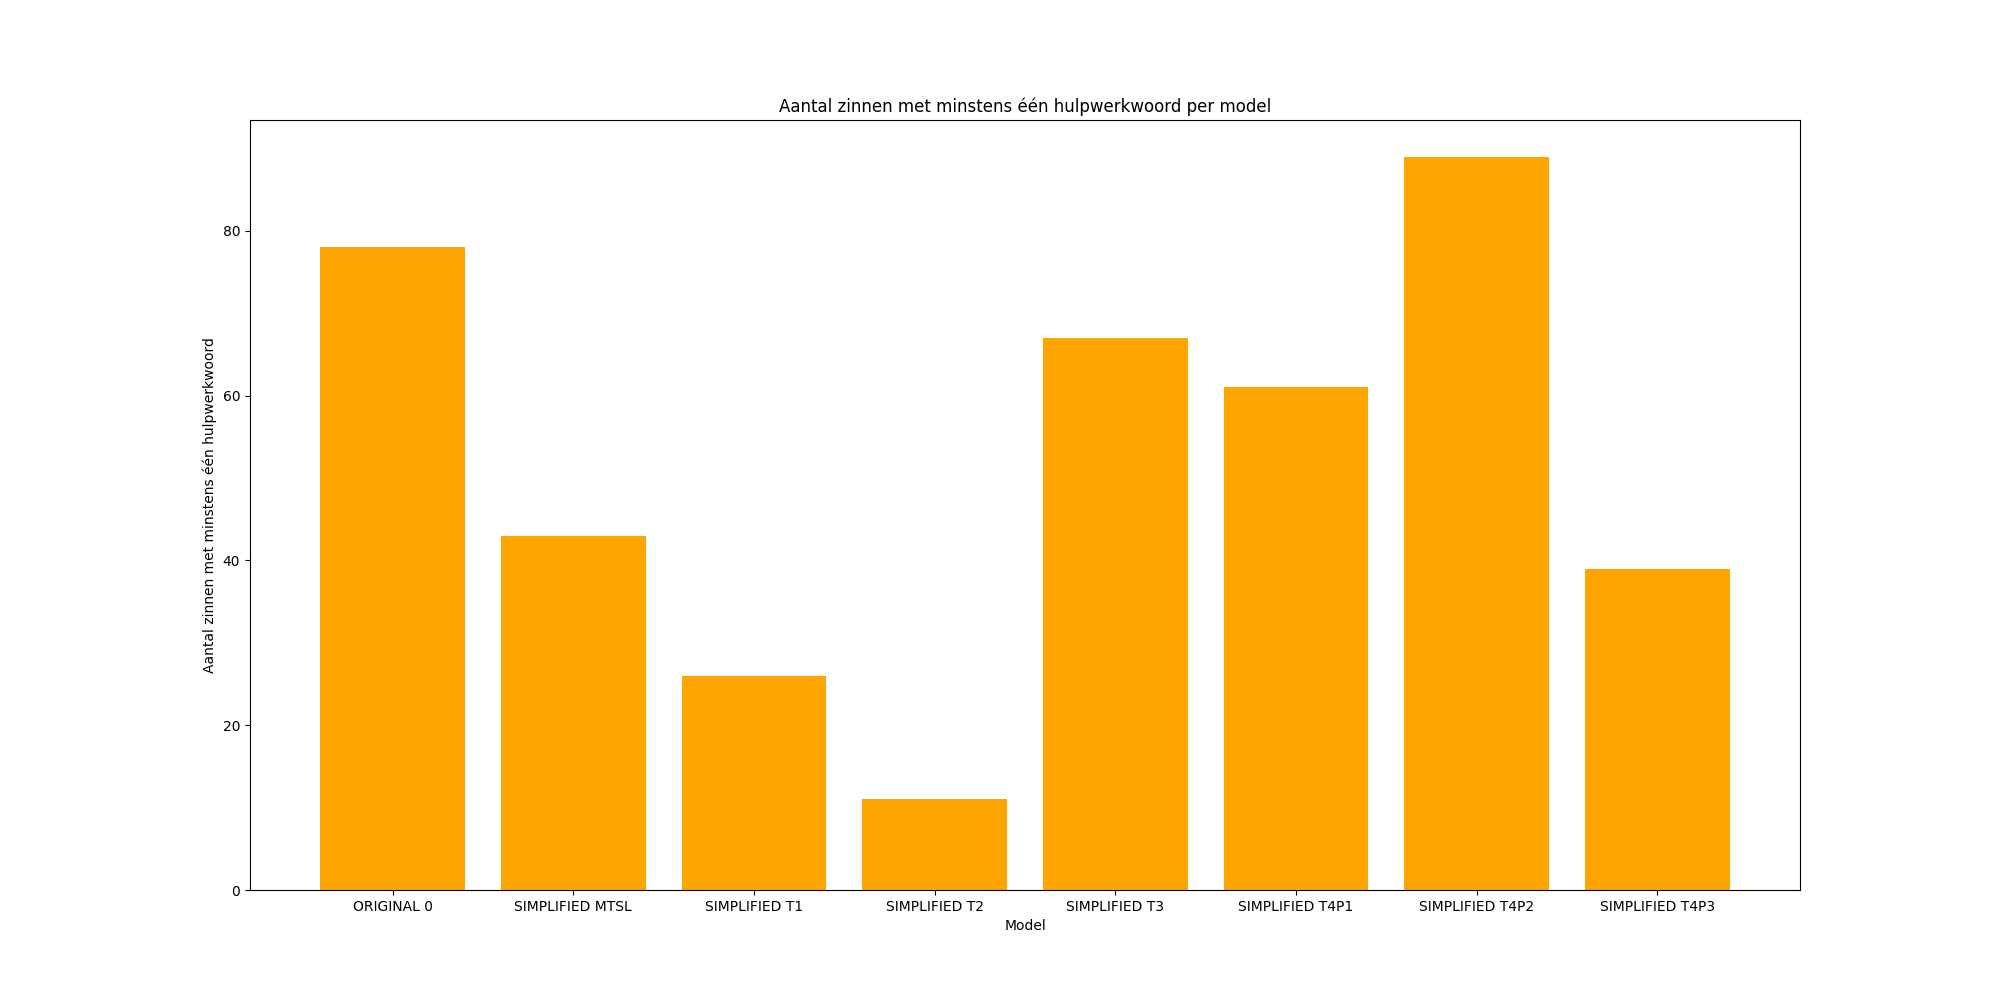
\includegraphics[width=\linewidth]{img/boxplot-aux-a1.png}
	\caption{Een staafdiagram van het aantal gebruikte hulpwerkwoorden in de tekst, gegroepeerd op model voor A1.}
	\label{img:histplot-aux-a1}
\end{figure}

\begin{figure}[H]
	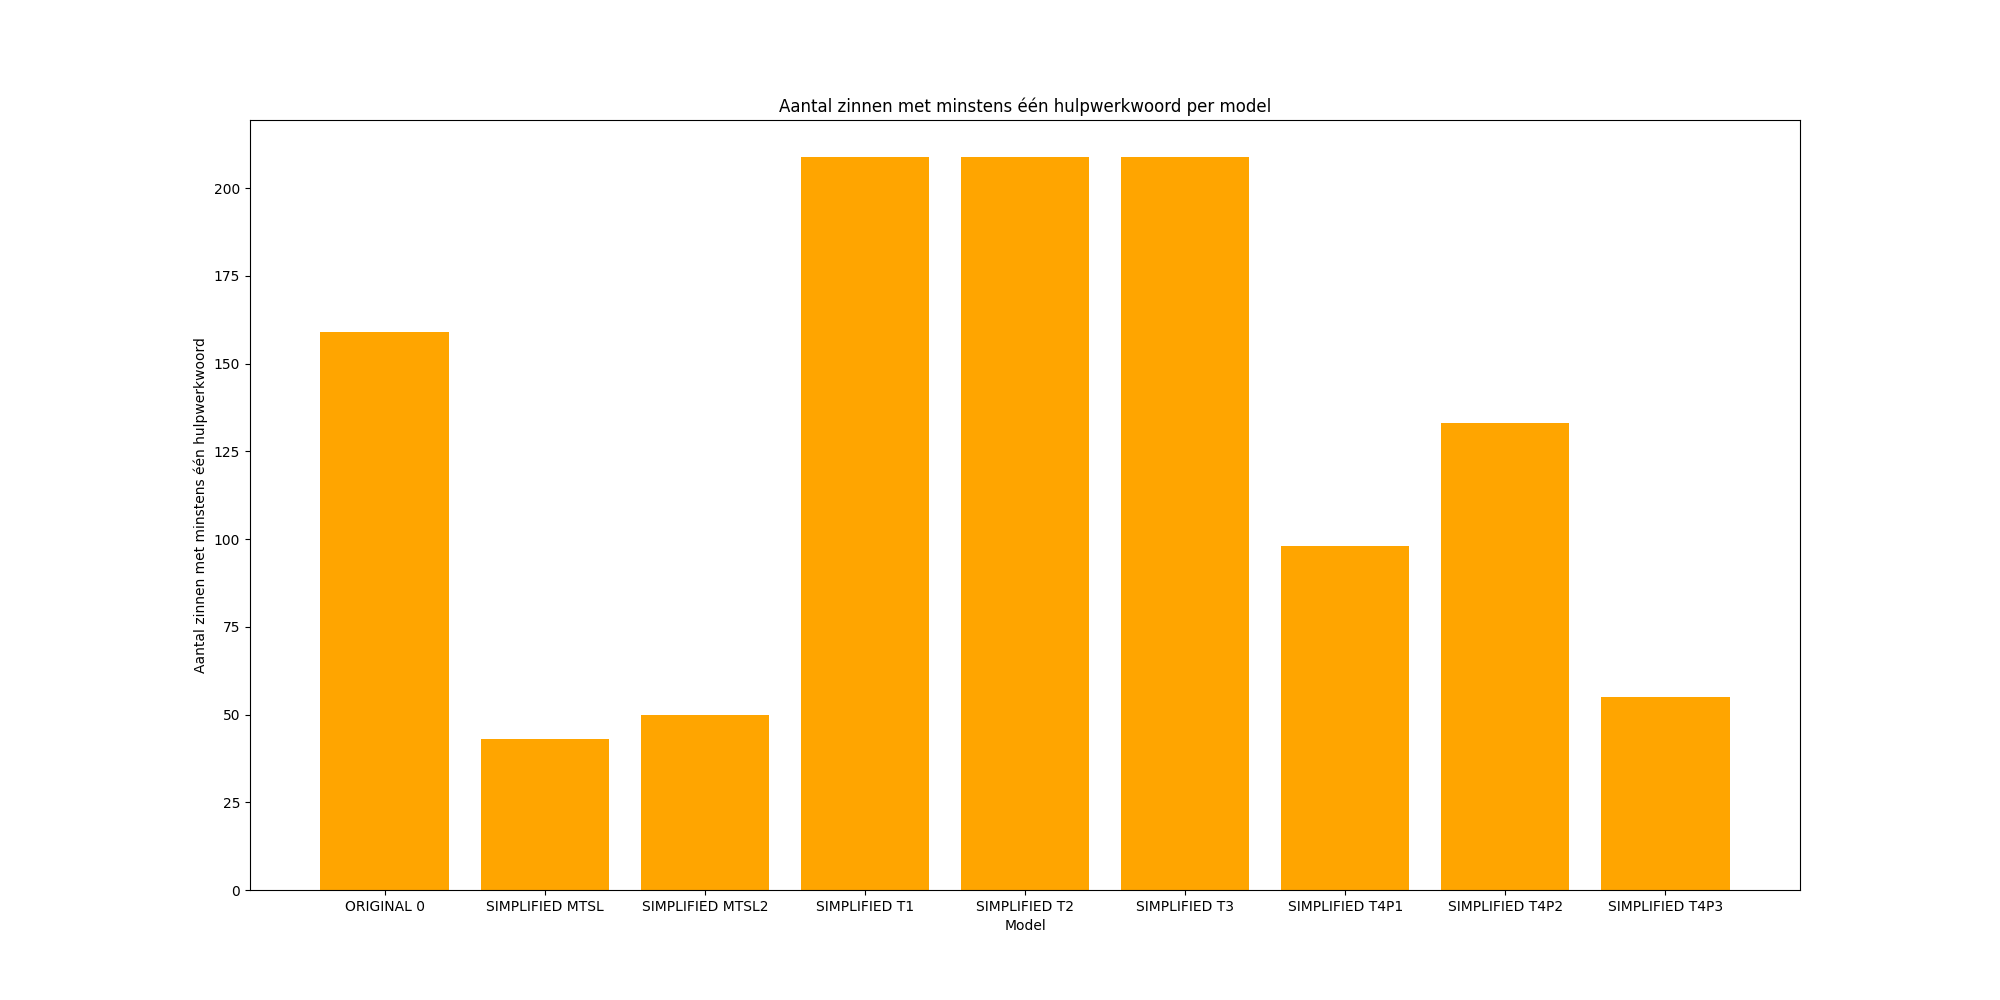
\includegraphics[width=\linewidth]{img/boxplot-aux-a2.png}
	\caption{Een staafdiagram van het aantal gebruikte hulpwerkwoorden in de tekst, gegroepeerd op model voor A2.}
	\label{img:histplot-aux-a2}
\end{figure}

\begin{figure}[H]
	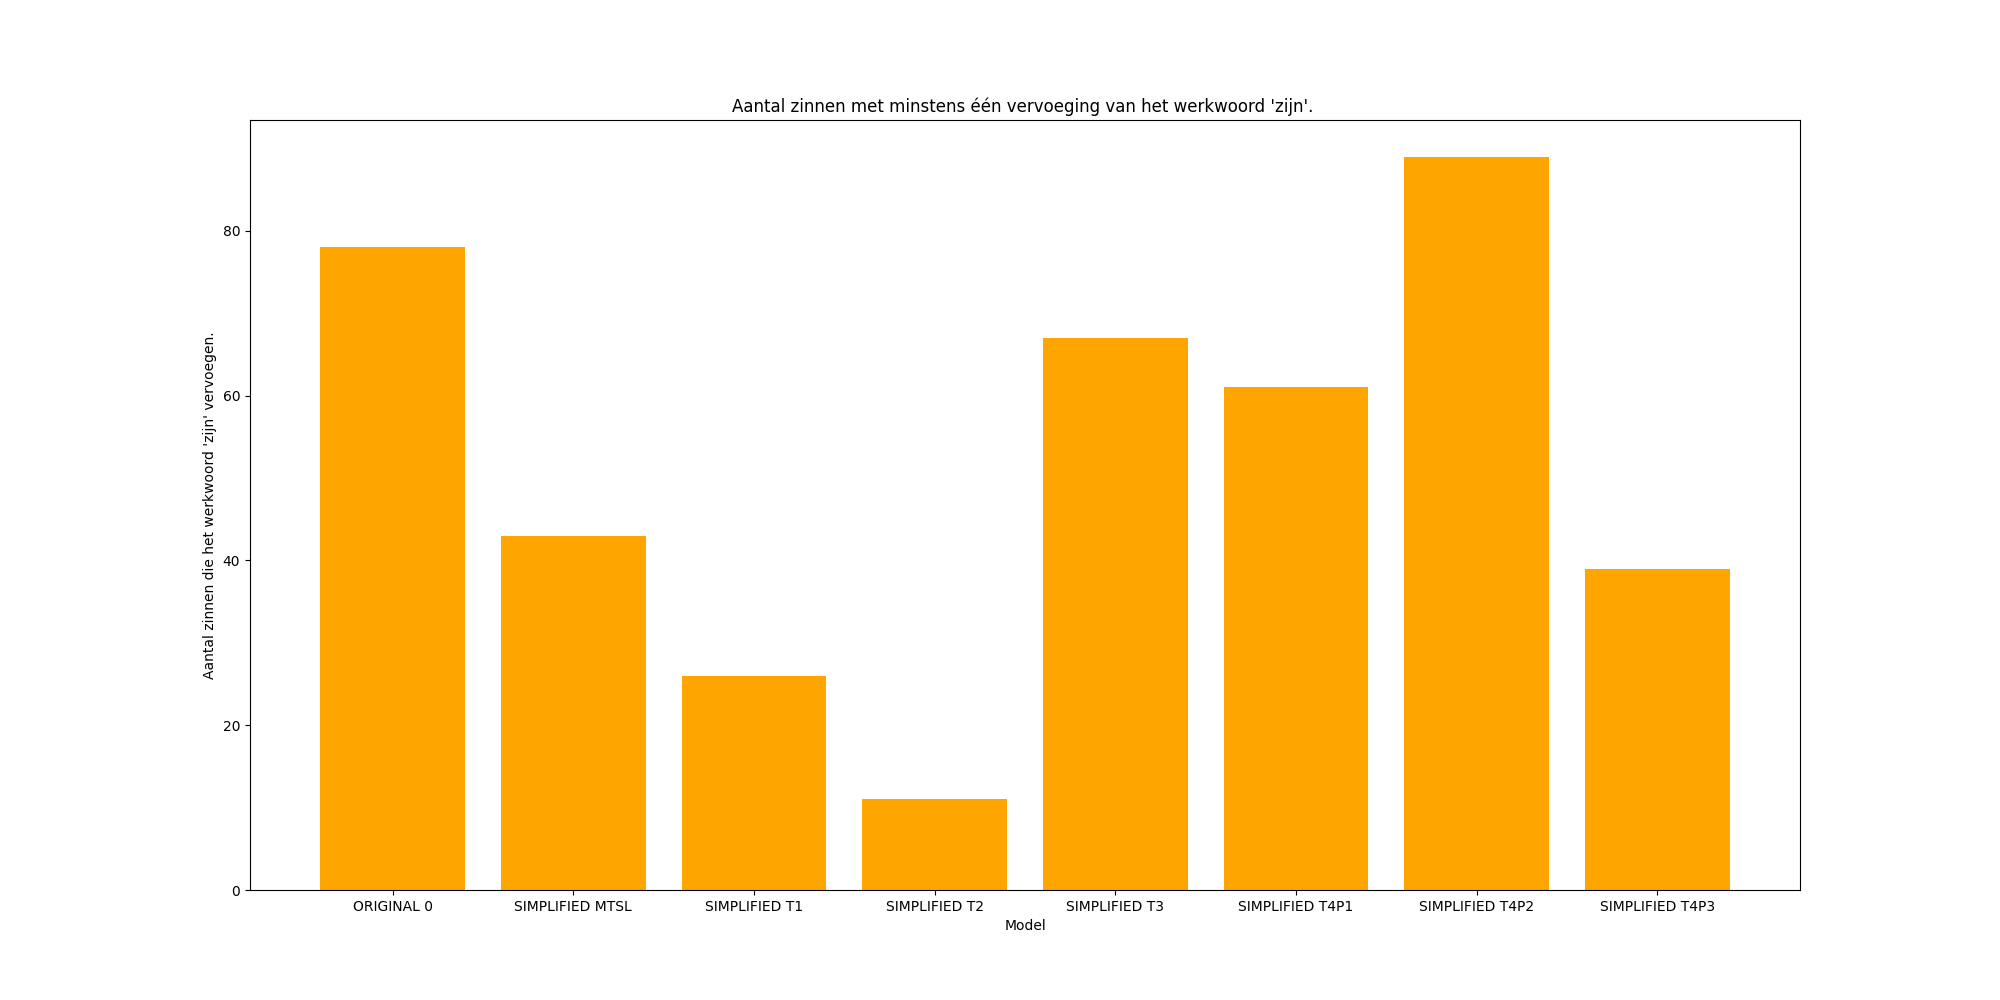
\includegraphics[width=\linewidth]{img/boxplot-tobe-a1.png}
	\caption{Het aantal vervoegingen van het werkwoord 'zijn', gegroepeerd op model voor A1.}
	\label{img:histplot-tobe-a1}
\end{figure}

\begin{figure}[H]
	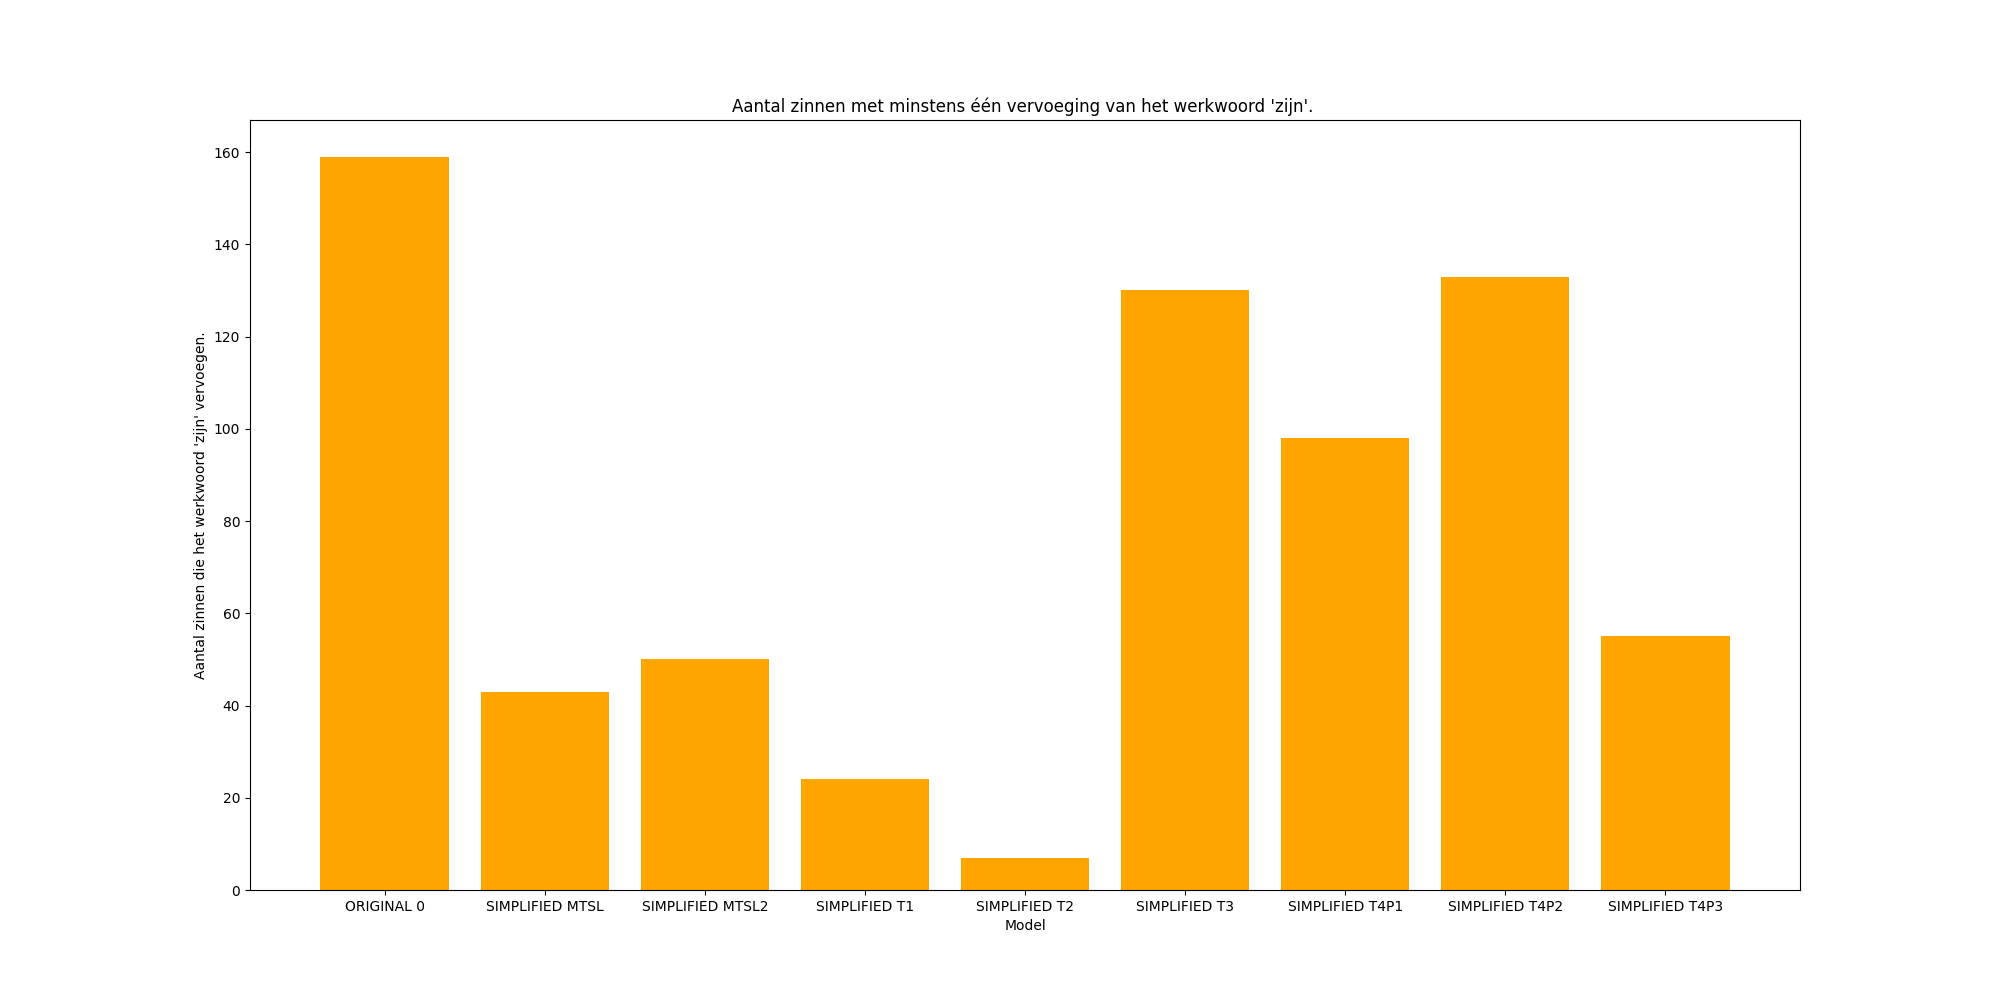
\includegraphics[width=\linewidth]{img/boxplot-tobe-a2.png}
	\caption{Het aantal vervoegingen van het werkwoord 'zijn', gegroepeerd op model voor A2.}
	\label{img:histplot-tobe-a2}
\end{figure}

\subsubsection{Menselijke beoordeling van de referentieteksten.}

In het volgende deel bespreekt het onderzoek de menselijke beoordeling van de resultaten. Allereerst kunnen T4P1 en T4P2 Engelstalige vaktermen vertalen naar het Nederlands. Zo blijft de afkorting voor 'DPKIA' intact, maar vertaalt T4P1 hetzelfde woord naar het Nederlands.  T1, T2, T3 en T4P3 houden hier echter geen rekening mee en behouden de oorspronkelijke versie van de tekst. De auteurs schrijven alle afkortingen voluit, zoals beschreven in de richtlijnen.

\medspace

Alle taalmodellen kunnen LS toepassen. De handmatig vereenvoudigde referentieteksten bevatten zinnen die vakjargon gebruiken op het niveau van 15 tot 18 jarige studenten. T4P1 kan uitleg tussen ronde haakjes schrijven, wanneer het geen eenvoudiger synoniem kan vinden. T4P1, T1, T2 en T3 passen woorden aan, maar schrijven geen extra uitleg. T4P3 past deze techniek minder toe dan de vooraf vermelde taalmodellen. T4P3 verkort lange zinnen door deze op te splitsen. T1, T2 en T3 behalen een gelijke zinslengte als dat van de oorspronkelijke zin. T4P1 en T4P2 kunnen langere zinnen genereren, maar smelten geen twee zinnen met elkaar samen. 

\medspace

Geen taalmodel wijkt af van de hoofdgedachte van het oorspronkelijke wetenschappelijk artikel. Hoewel T1, T2 en T3 deels afgebroken zinnen kan genereren, bevatten deze zinnen de hoofdgedachte. T2 bevat minder dan 10\% van het oorspronkelijk artikel en ontbreekt daarbij bijzaken die nodig zijn om alle vragen in \ref{ch:referentietekst} te kunnen begrijpen en te beantwoorden. Tenslotte verwerken T1, T2 en T3 de APA- en California bronvermeldingen niet in de vereenvoudigde teksten. Hoewel T4 deze wel verwerkt, bevat de tekst na een vereenvoudiging deze bronvermeldingen niet meer.

\medspace

Ter conclusie van de resultaten scoren de drie prompts van T4 beter bij de menselijke beoordeling van de resultaten. Het taalmodel en de verwante drie prompts genereren coherente teksten met een verlaagde lexicale complexiteit. Echter houden de geteste taalmodellen weinig tot geen rekening met afkortingen of bronvermeldingen.

\section{Het prototype voor tekstvereenvoudiging met ATS vergeleken met top-of-the-line tools.}

% deelvraag: Hoe kan een intuïtieve en lokale webtoepassing worden ontwikkeld die zowel scholieren met dyslexie als docenten helpt bij het vereenvoudigen van wetenschappelijke artikelen met behoud van semantiek, jargon en zinsstructuren?

Gebruikers kunnen vanuit de homepagina drie schermen kiezen: het lerarencomponent, het scholierencomponent en een instellingenpagina. In de instellingenpagina kunnen eindgebruikers de opmaakopties aanpassen naargelang hun keuze. Figuur \ref{img:website-instellingen} toont alle aanpasbare opmaakopties die het prototype aanreikt.

\begin{center}
	\begin{figure}[H]
		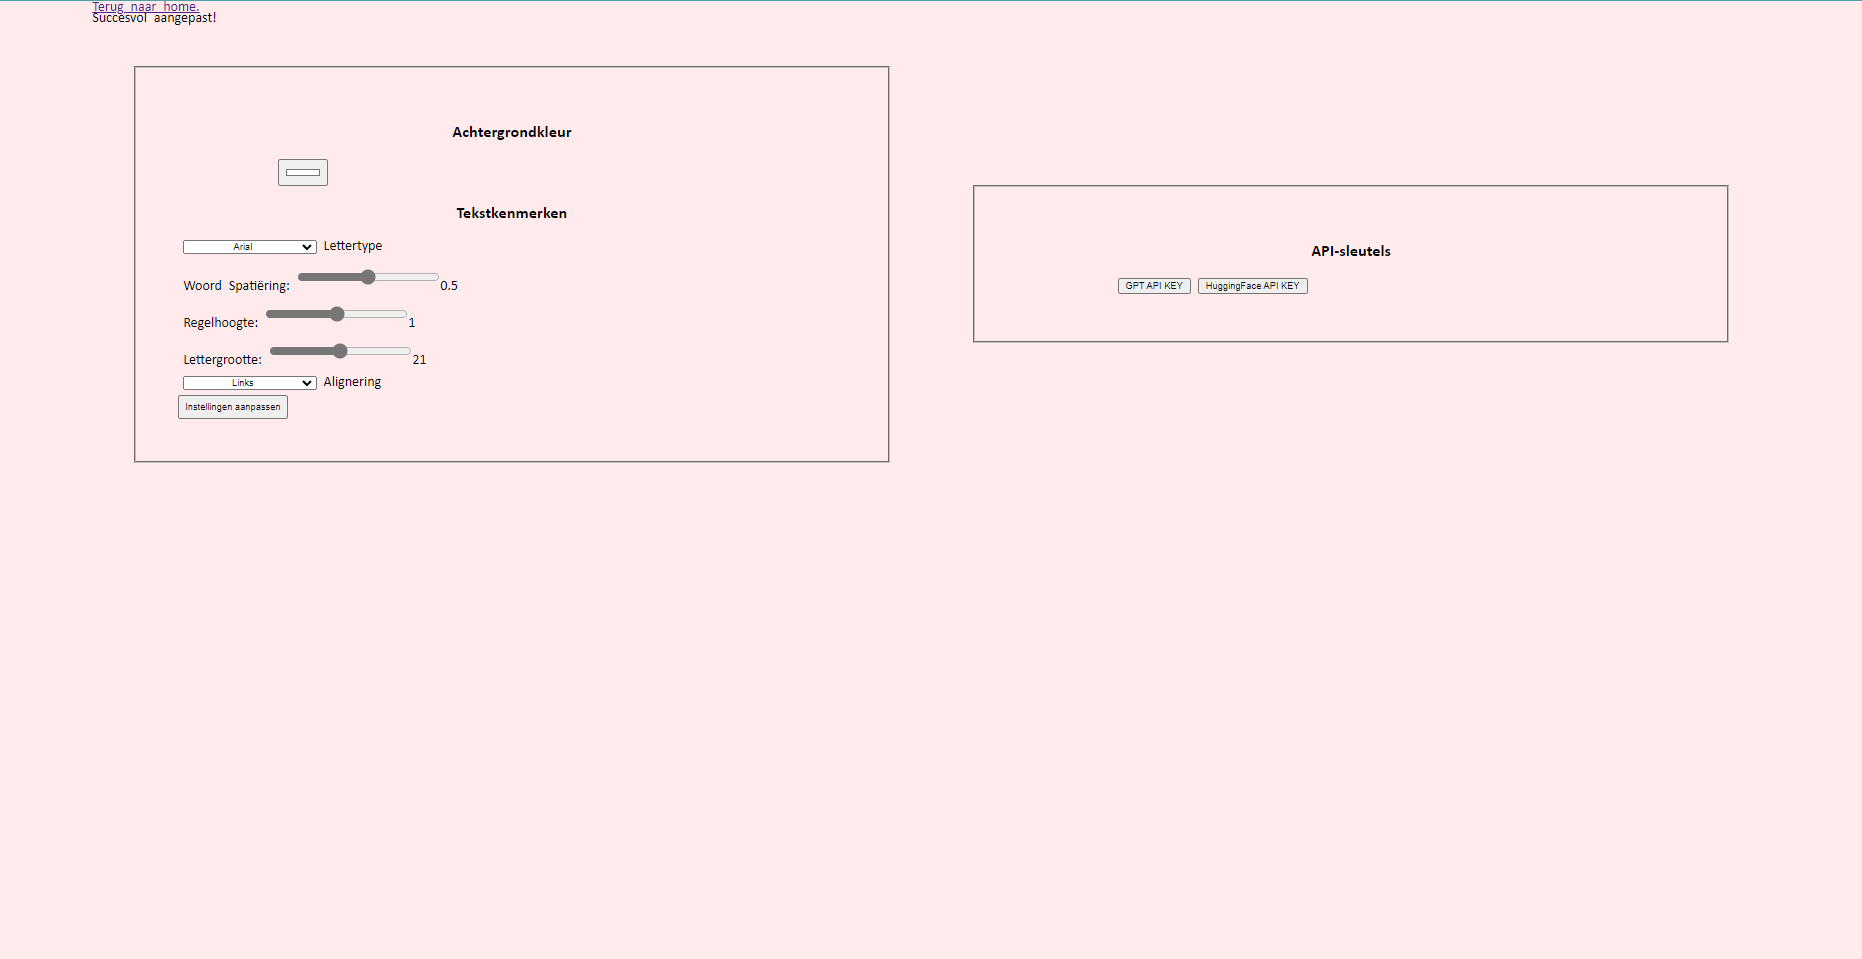
\includegraphics[width=\linewidth]{img/website-instellingen.png}
		\caption{Voorbeeldweergave van de instellingenpagina.}
		\label{img:website-instellingen}
	\end{figure}
\end{center}

Bovendien stelt het prototype gebruikers in staat om op basis van gekregen parameters automatisch personaliseerbare pdf en docx-documenten te genereren.

\begin{figure}[H]
	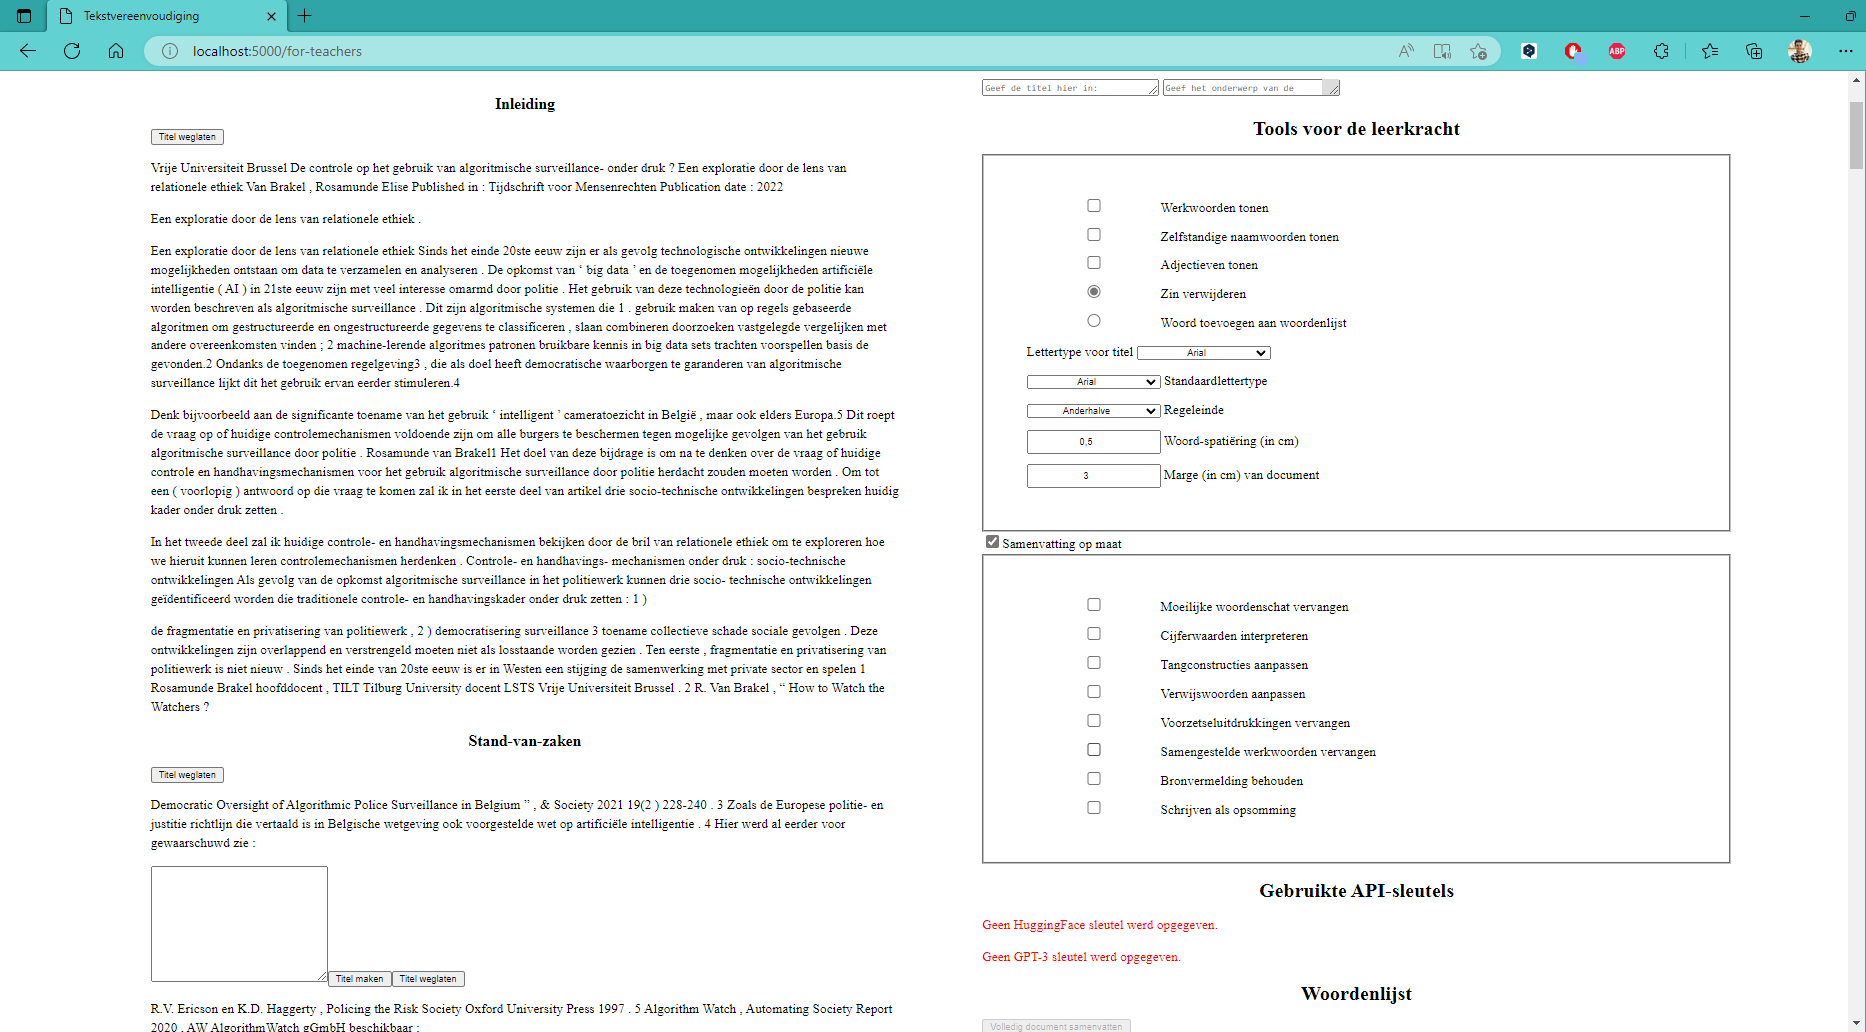
\includegraphics[width=\linewidth]{img/proto-lerarencomponent.png}
	\caption{Een mogelijke weergave van het lerarencomponent met het wetenschappelijk artikel van \textcite{VanBrakel2022} als input.}
	\label{img:proto-lerarencomponent}
\end{figure}

\begin{center}
	\begin{figure}[H]
		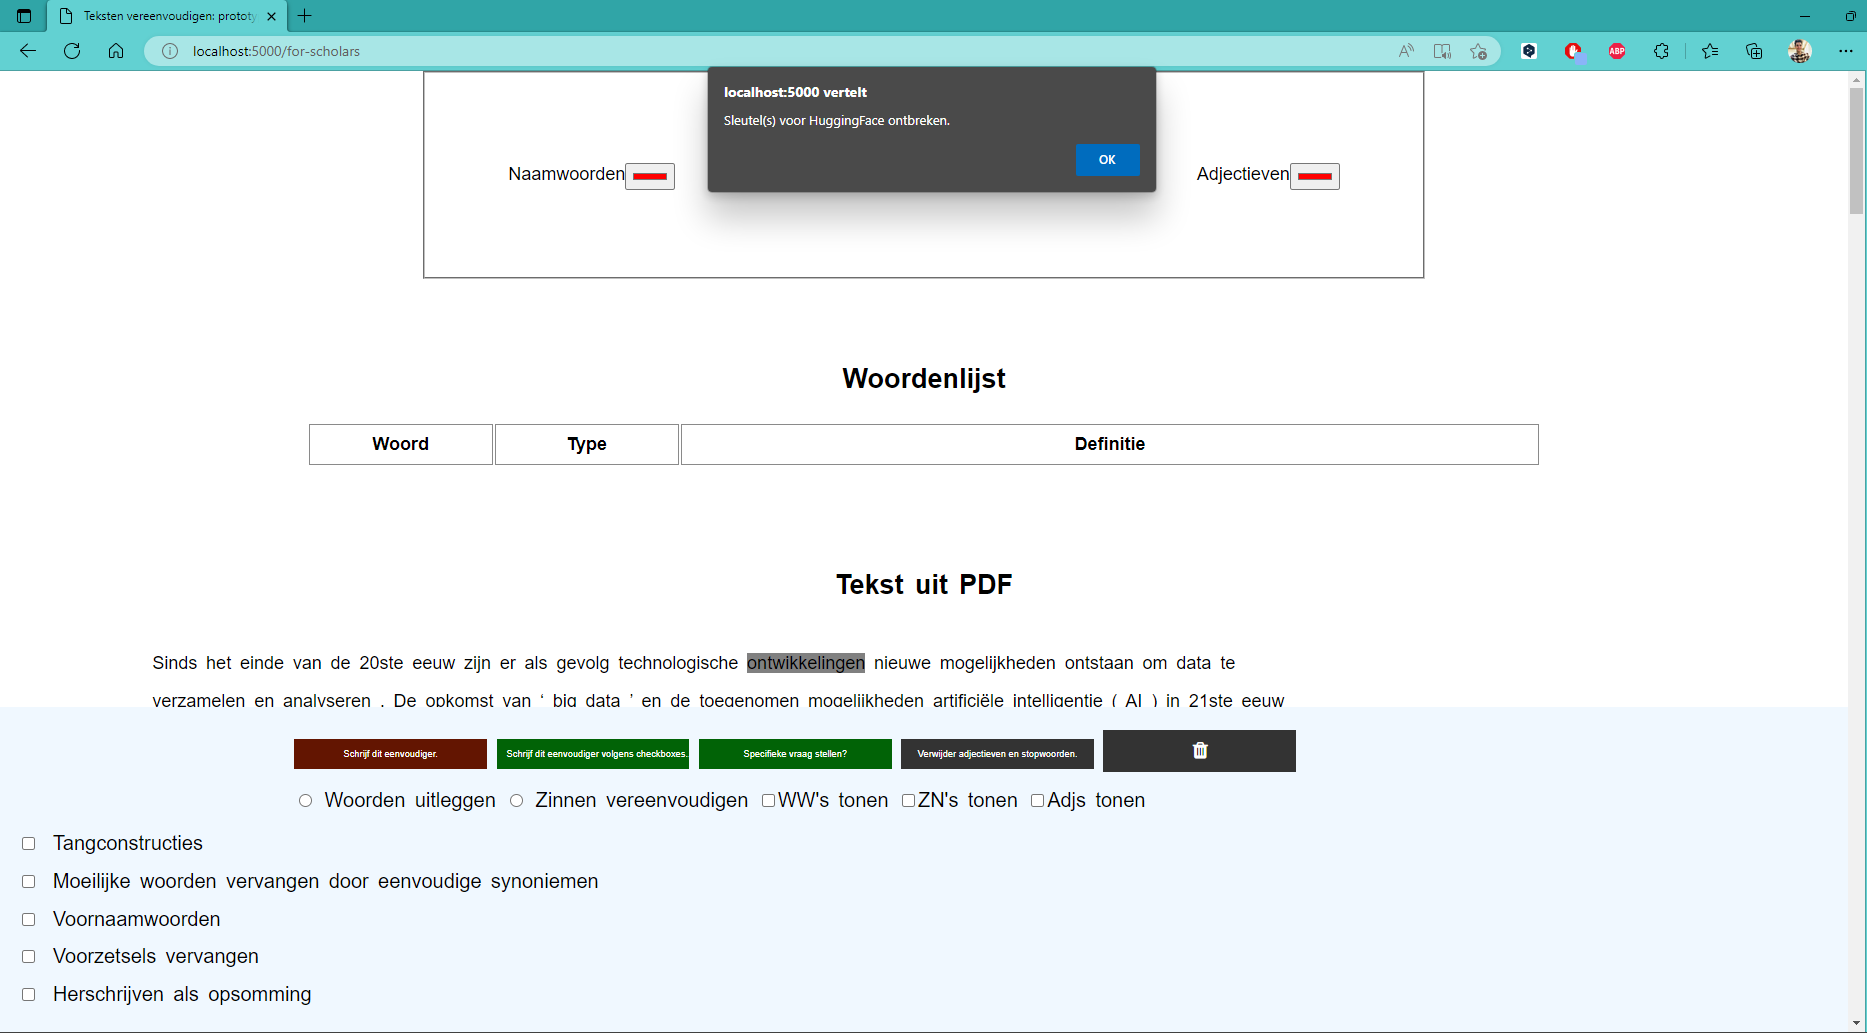
\includegraphics[width=\linewidth]{img/proto-melding.png}
		\caption{Een voorbeeldweergave van het scholierencomponent.}
		\label{img:proto-homescreen-scholieren}
	\end{figure}
\end{center}

Figuur \ref{img:proto-pos-tagging-scholieren} toont een voorbeeldweergave van deze functionaliteit. 

\begin{center}
	\begin{figure}[H]
		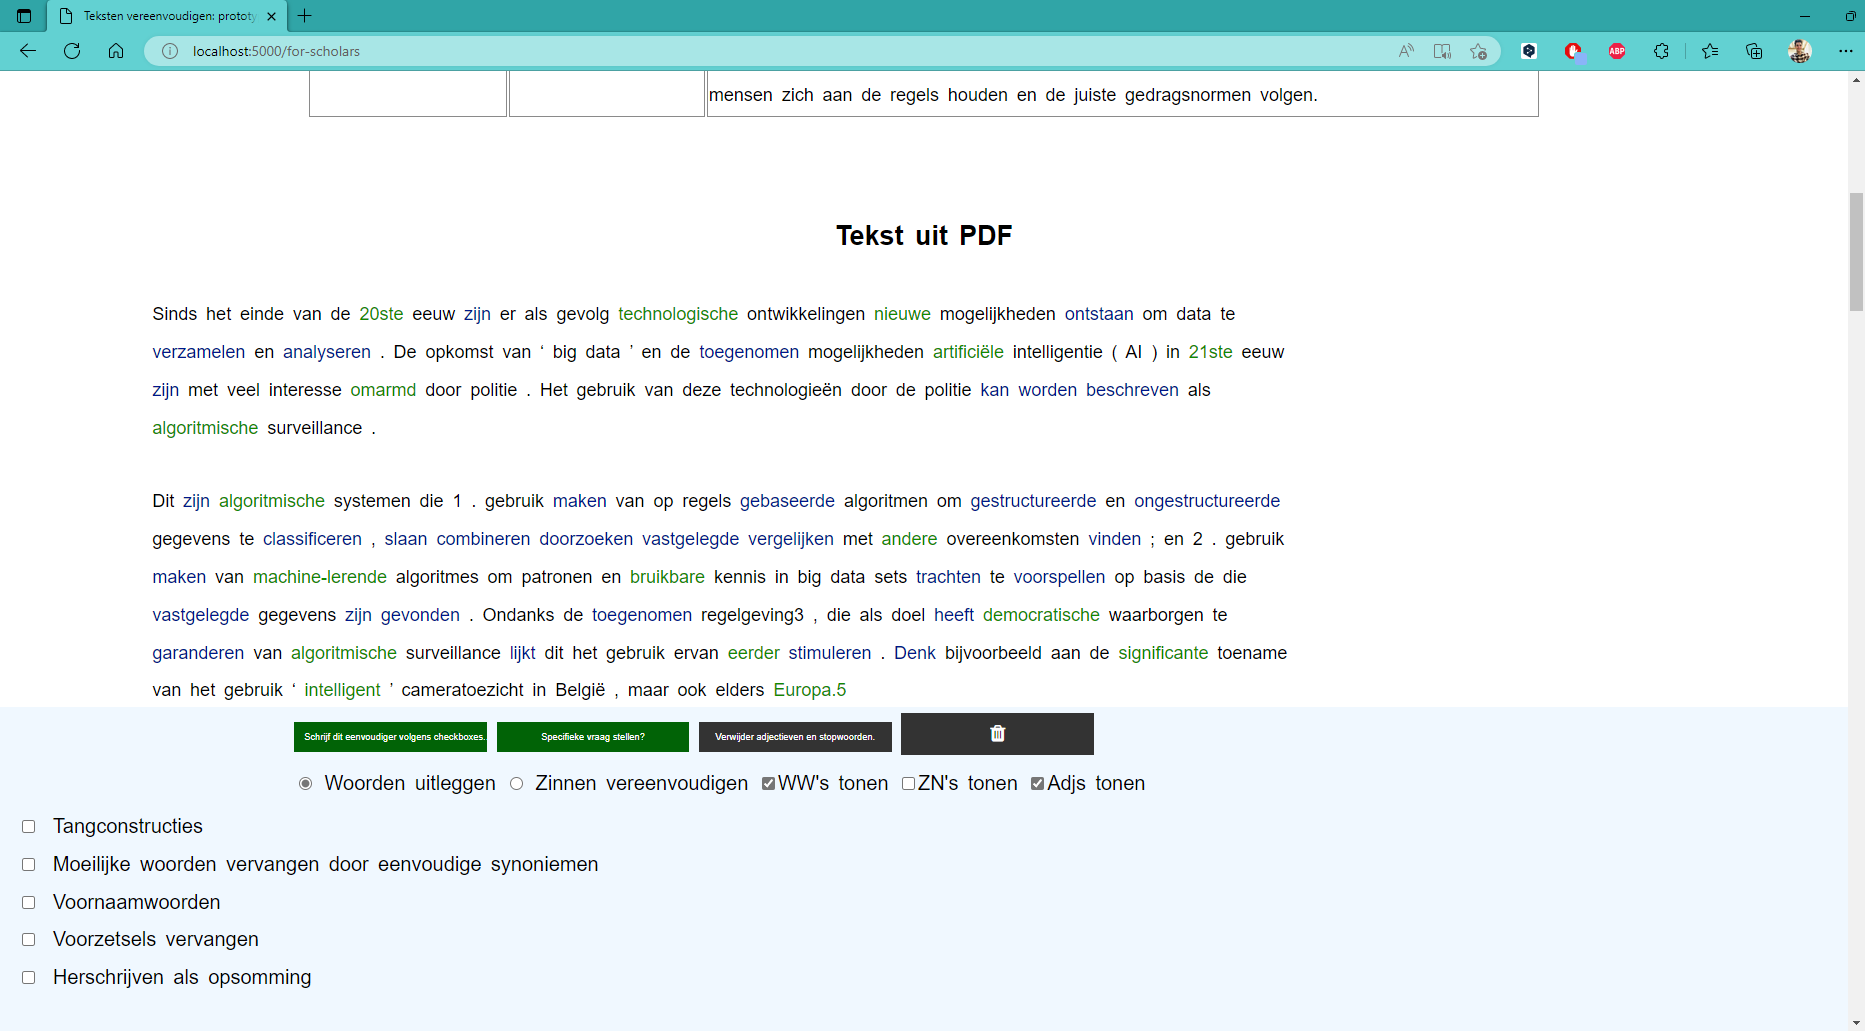
\includegraphics[width=\linewidth]{img/proto-pos-tagging.png}
		\caption{Een voorbeeldweergave van de toepassing van PoS-tagging bij het scholierencomponent.}
		\label{img:proto-pos-tagging-scholieren}
	\end{figure}
\end{center}

Scholieren kunnen zinnen selecteren om daarna deze tekst te laten vereenvoudigen met gepersonaliseerde ATS. Figuren \ref{img:proto-scholieren-step-1} en \ref{img:proto-scholieren-step-3} tonen hoe een gebruiker van gemarkeerde doorlopende tekst een opsomming kan maken met het prototype. Het prototype kan doorlopende tekst omvormen naar een opsomming van tekst. Echter beschikt het prototype geen functionaliteit om doorlopende tekst naar een tabel om te vormen.

\begin{center}
	\begin{figure}[H]
		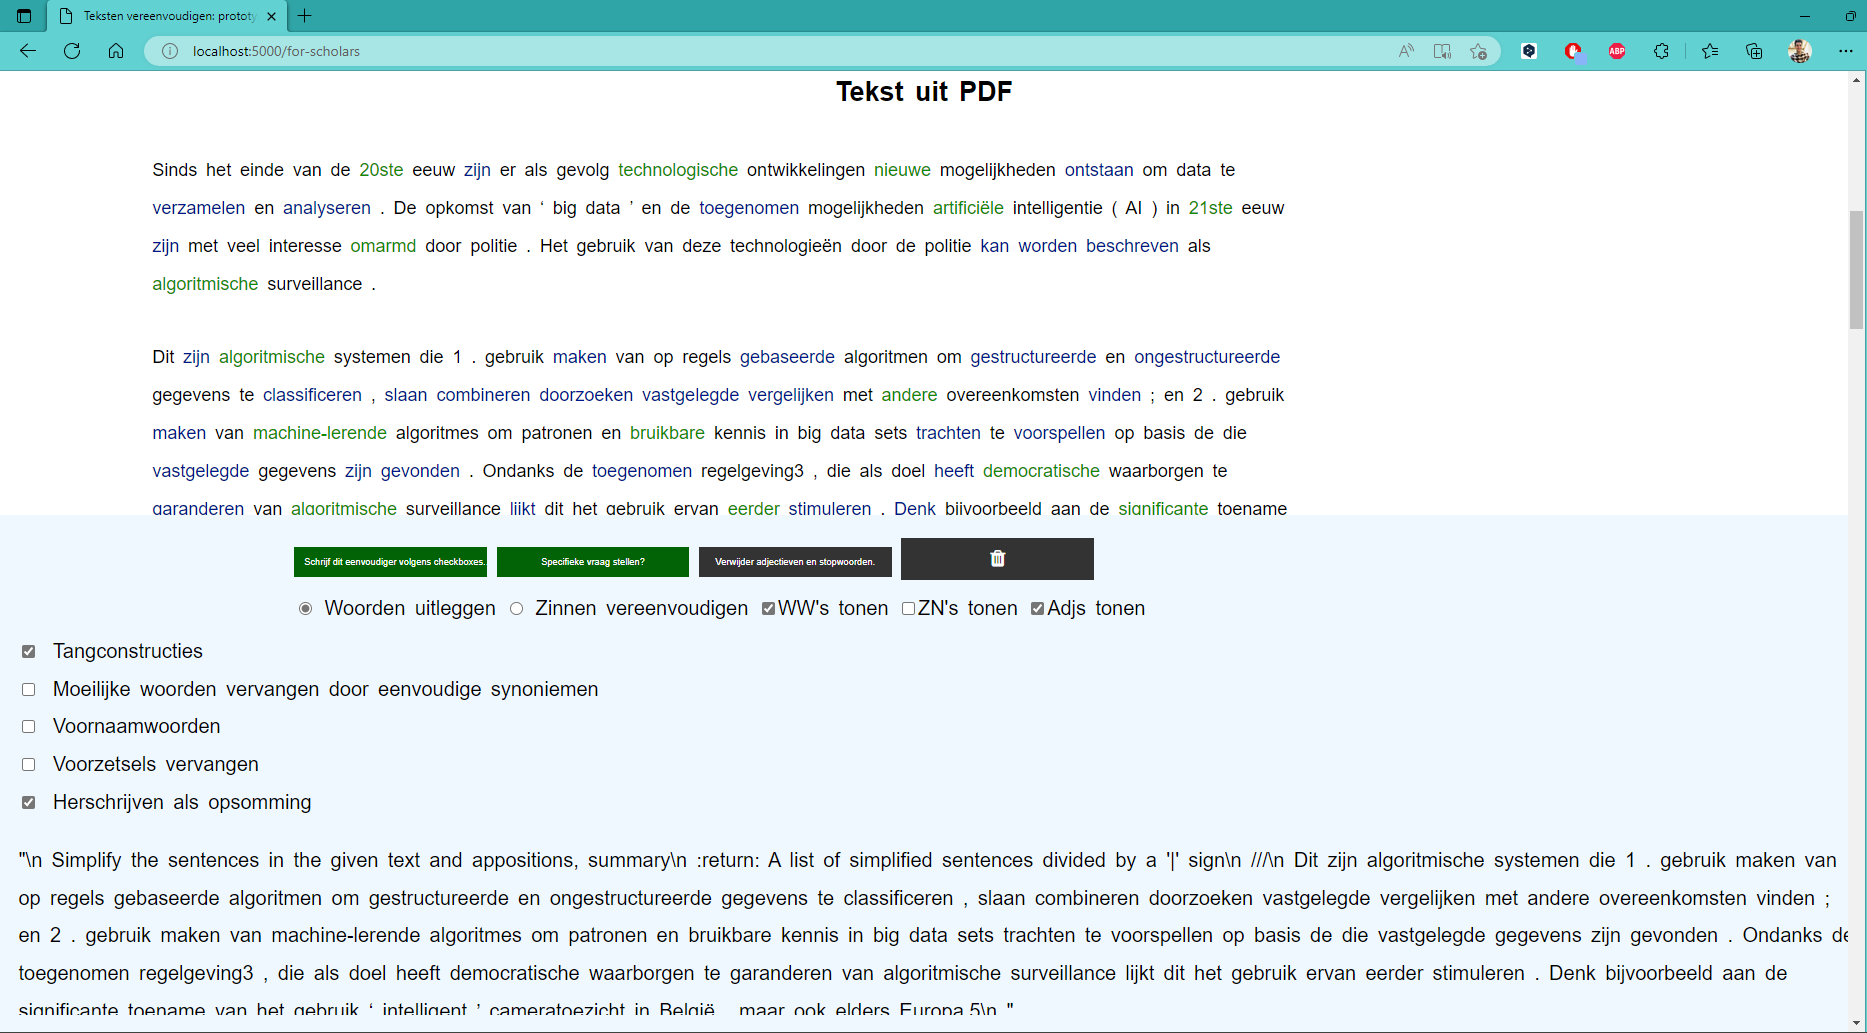
\includegraphics[width=\linewidth]{img/proto-opsomming-1.png}
		\caption{Stap 1 van een gepersonaliseerde tekstvereenvoudiging in het scholierencomponent.}
		\label{img:proto-scholieren-step-1}
	\end{figure}
\end{center}

\begin{center}
	\begin{figure}[H]
		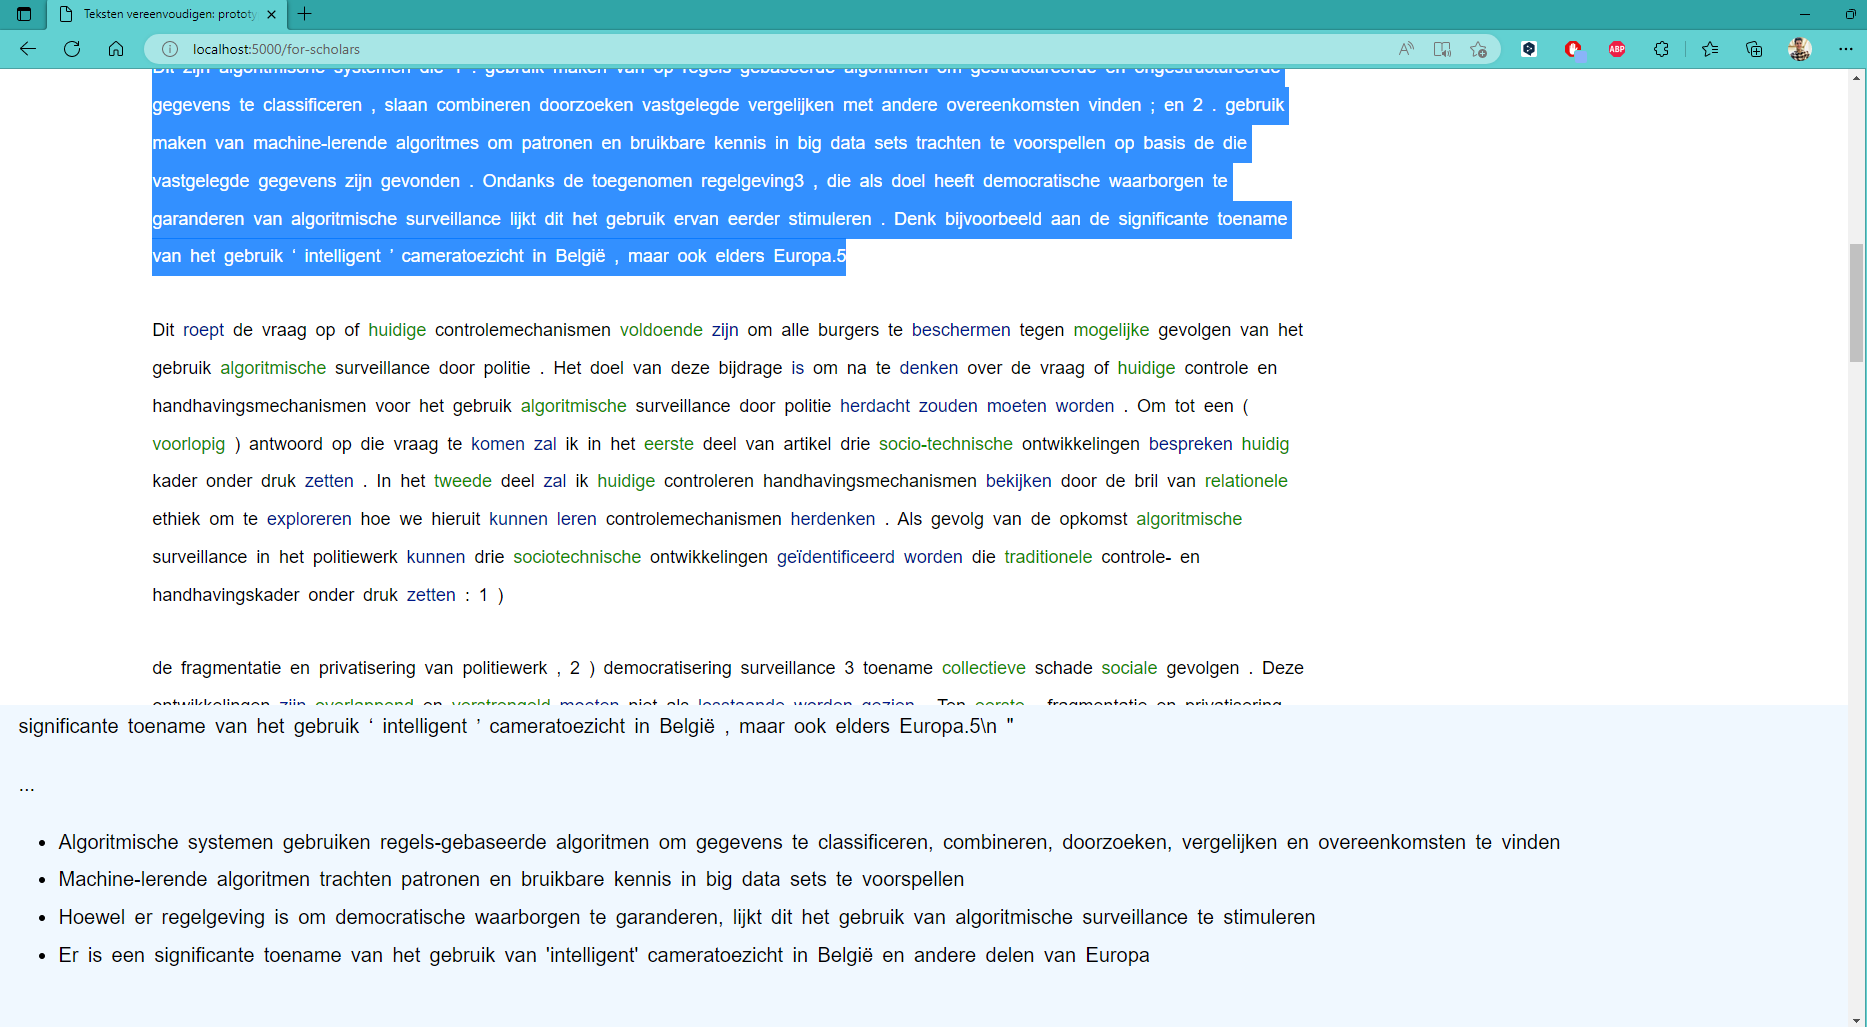
\includegraphics[width=\linewidth]{img/proto-opsomming-3.png}
		\caption{Stap 2 van een gepersonaliseerde tekstvereenvoudiging in het scholierencomponent.}
		\label{img:proto-scholieren-step-3}
	\end{figure}
\end{center}

Figuren \ref{img:step-1-proto-vraagstelling} en \ref{img:step-2-proto-vraagstelling} tonen een tweede functionaliteit. Zo kunnen scholieren specifieke vragen stellen aan het prototype door middel van een gecentreerd invoerscherm.

\begin{center}
	\begin{figure}[H]
		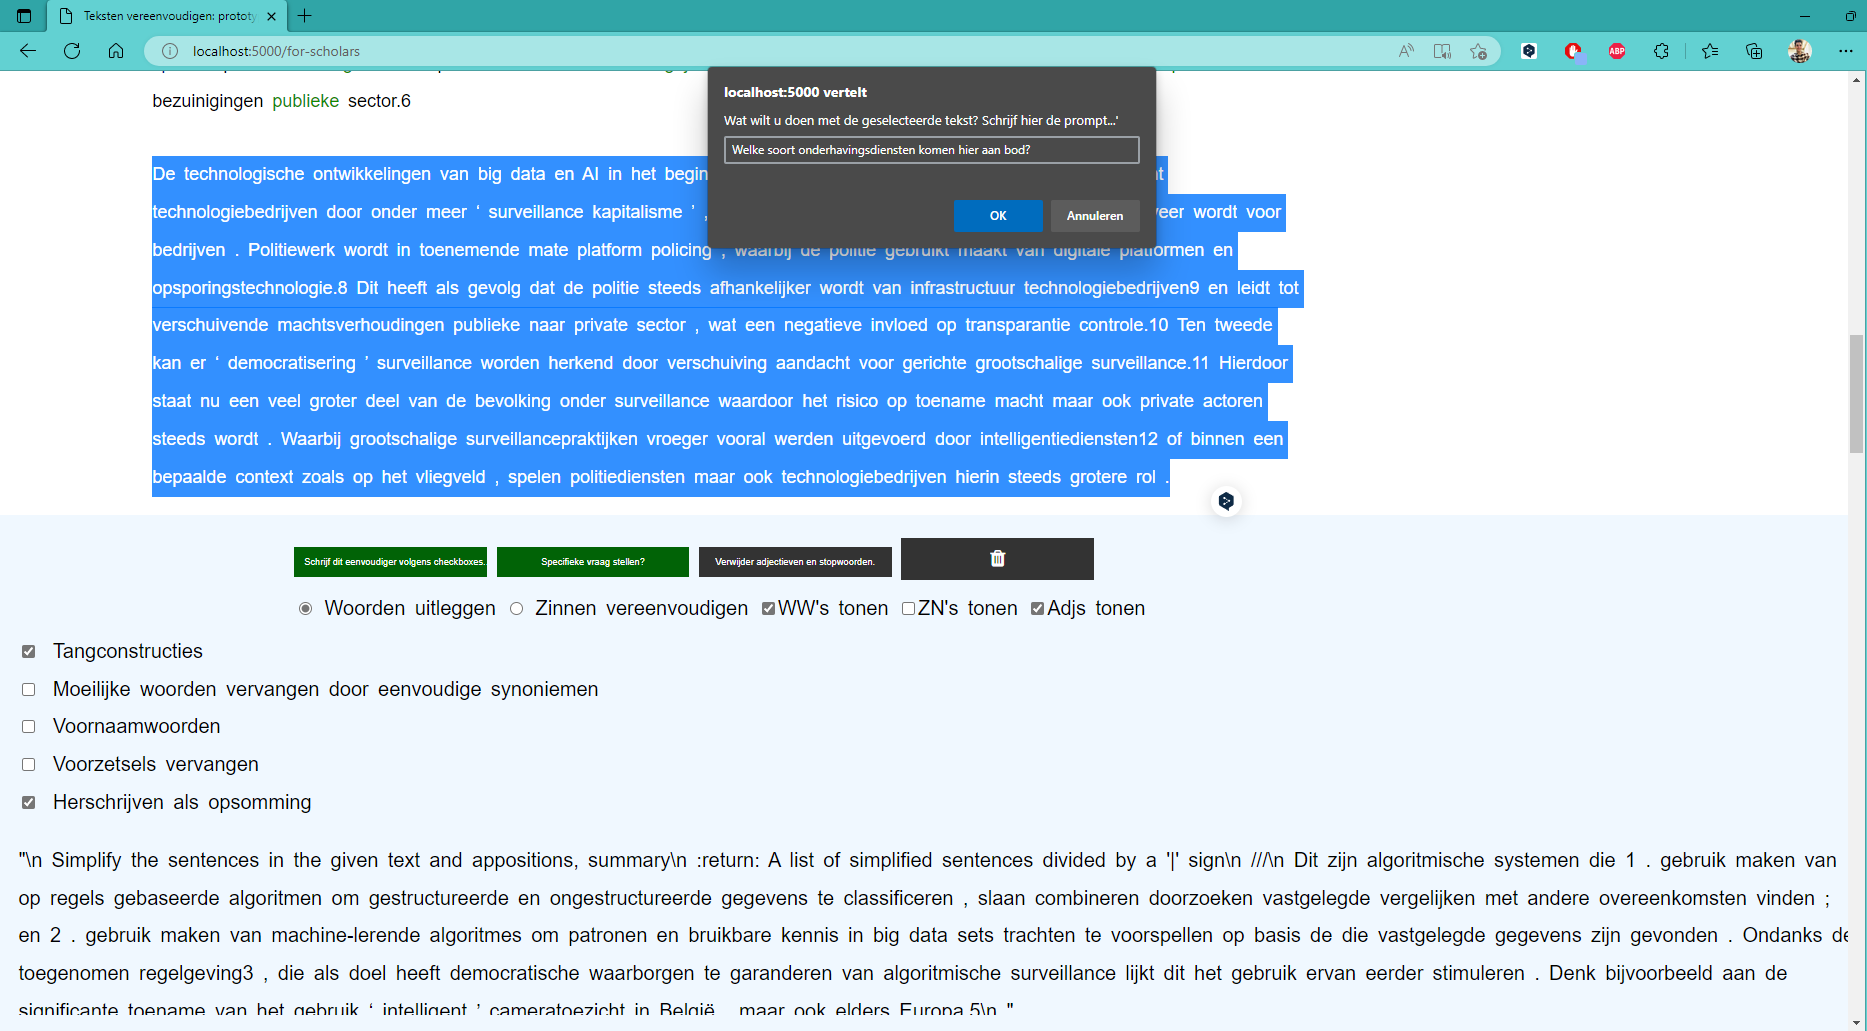
\includegraphics[width=\linewidth]{img/proto-vraagstelling-1.png}
		\caption{Stap 1 bij het stellen van een specifieke vraag bij gemarkeerde tekst.}
		\label{img:step-1-proto-vraagstelling}
	\end{figure}
\end{center}

\begin{center}
	\begin{figure}[H]
		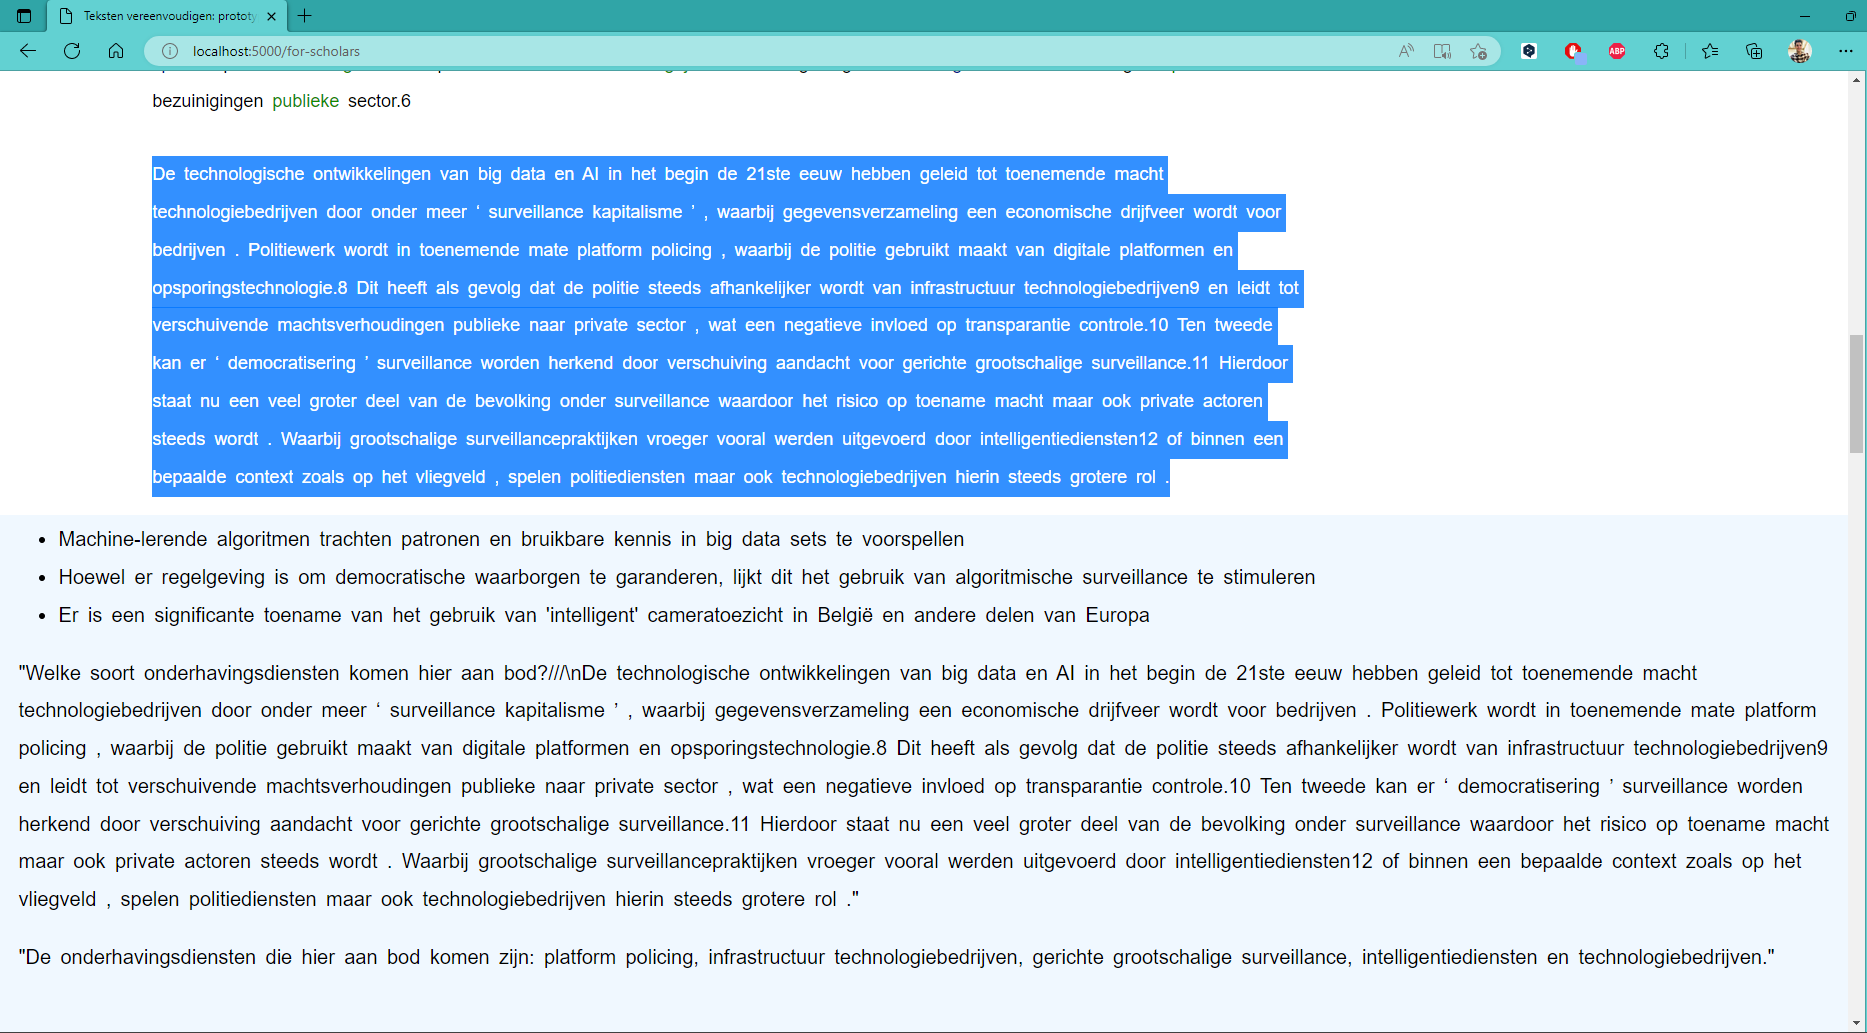
\includegraphics[width=\linewidth]{img/proto-vraagstelling-2.png}
		\caption{Stap 2 bij het stellen van een specifieke vraag bij gemarkeerde tekst.}
		\label{img:step-2-proto-vraagstelling}
	\end{figure}
\end{center}

Na evaluatie en experimenten blijkt het prototype te voldoen aan de \textit{must-have} functionaliteiten, zoals vastgesteld in het moscow-schema of tabel \ref{img:moscow-table}. Zo biedt het prototype twee manieren aan om pdf-bestanden in te lezen, namelijk via OCR en via PDFMiner. Daarnaast kan \textit{plain-text} ook dienen als voer voor het prototype. Dit valt in lijn met de verwachtte functionaliteiten omtrent pdf-upload. Tot slot kunnen gebruikers kiezen welke tekstinhoud zij willen vereenvoudigen met gepersonaliseerde ATS. De eindgebruiker kan alle vragen beantwoorden met de inhoud van het vereenvoudigde artikel, zoals aangegeven door \textcite{Hollenkamp2020} als absolute must na de vereenvoudiging of samenvatting van een wetenschappelijk artikel.

\medspace

Alle eindgebruikers kunnen de opmaakopties van de toepassing aanpassen aan hun persoonlijke voorkeuren bij het lezen van wetenschappelijke artikelen. Alsook de opmaak van het uitvoerbestand personaliseren. Figuur \ref{img:screenshot-pdf-attempt} toont de vereenvoudigde versie van het wetenschappelijke artikel met de parameters uit tabel \ref{table:chosen-parameters-experiment}. Het prototype kan de regeleindes, woord- en karakterspatiëring, lettertype -en grootte, koppenstructuur en marges van het uitvoerbestand aanpassen. Deze functionaliteit is niet beschikbaar bij de uitgeteste tools, behalve E1 en E2 die enkel het lettertype -en grootte kan aanpassen. 

\begin{figure}[H]
	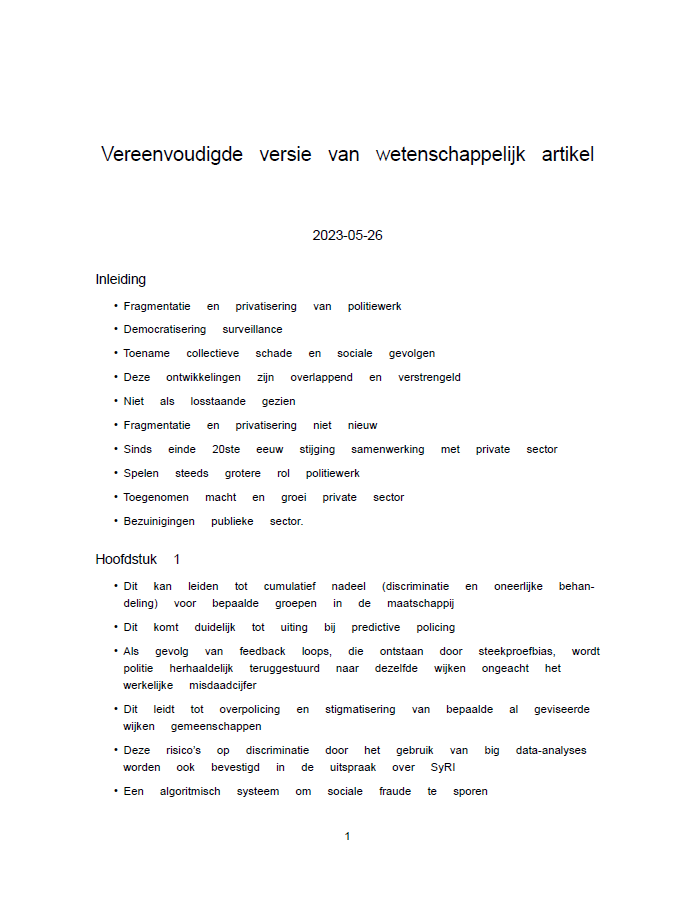
\includegraphics[width=\linewidth]{img/screenshot-prototype-pdf.png}
	\caption{Een vereenvoudigde versie in pdf-formaat van het artikel van \textcite{VanBrakel2022} volgens het prototype.}
	\label{img:screenshot-pdf-attempt}
\end{figure}

Figuur \ref{img:screenshot-docx-attempt} illustreert hoe het prototype niet in staat is om een volledig personaliseerbare docx-bestand te maken. Het prototype maakt geen gebruik van de meegegeven woordspatiëring. Lettertype- en grootte, documentmarge en regeleindes past het prototype wel aan.

\begin{figure}[H]
	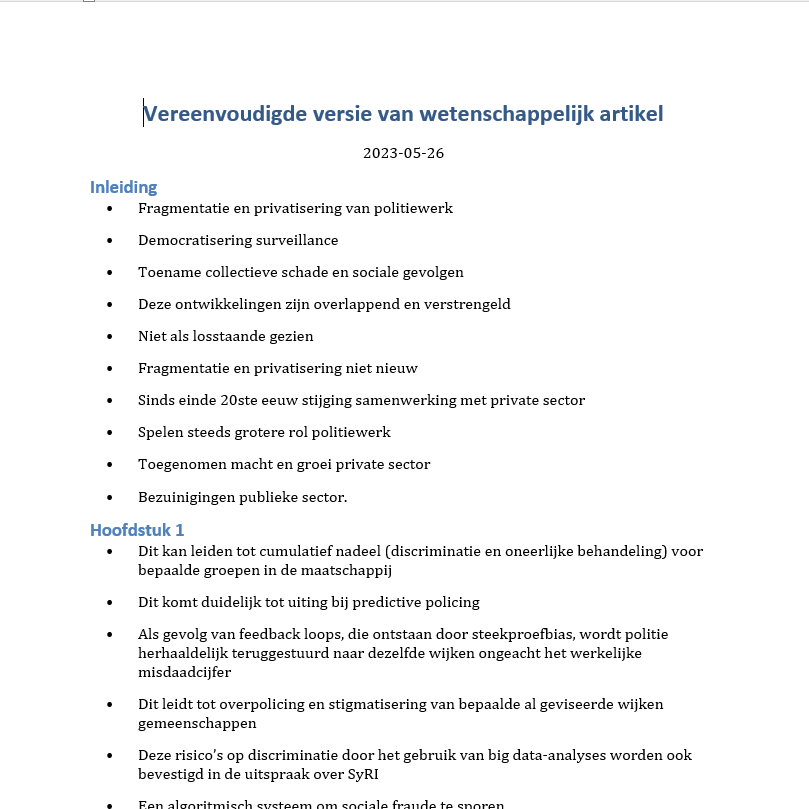
\includegraphics[width=\linewidth]{img/screenshot-prototype-word.png}
	\caption{Een vereenvoudigde versie in docx-formaat van het artikel van \textcite{VanBrakel2022} volgens het prototype.}
	\label{img:screenshot-docx-attempt}
\end{figure}

Het prototype beschikt over enkele van de \textit{should-haves}. Zo geeft het prototype geen tekstanalyse aan de eindgebruiker. Door middel van eenduidige handelingen kunnen de eindgebruikers zinnen markeren. Het prototype kan de zin aanpassen door een \textit{in-line} definitie toe te voegen. Vervolgens beschikt het prototype over enkele \textit{could-haves}. Allereerst maakt het prototype geen gebruik van expliciete extraherende of abstraherende samenvatting. Abstraherende samenvatting bestaat echter wel in de vorm van een opsomming, zoals aangewezen in figuur \ref{img:screenshot-pdf-attempt} en \ref{img:screenshot-docx-attempt}. Vervolgens geeft het prototype een gefixeerd meldingscherm wanneer het prototype iets van de gebruiker verwacht, zoals aangegeven in figuur \ref{img:step-1-proto-vraagstelling}. Daarnaast geeft het prototype ook waarschuwingen in de formulieren aan de gebruiker, zoals weergegeven in figuur \ref{img:proto-lerarencomponent}. Tot slot is er geen functionaliteit om automatisch een woordenlijst met moeilijke woorden of vakjargon aan te maken.

\medspace

Tot slot bevat het prototype geen \textit{wont-haves}. Zo ontbreekt het prototype een luistercomponent waarbij scholieren de vereenvoudigde tekst kunnen beluisteren. Deze functionaliteit is wel aanwezig bij E1, E2 en E3. Daarnaast is het prototype niet beschikbaar als browserextensie. Andere uitgeteste tools beschikken hier ook niet over. Tot slot is het prototype enkel in een lokale omgeving beschikbaar. Andere uitgeteste toepassingen zijn online beschikbaar. 